% \iffalse meta-comment
%
% Copyright (C) 2017--2019 by Xiangdong Zeng <xdzeng96@gmail.com>
%
% This work may be distributed and/or modified under the
% conditions of the LaTeX Project Public License, either
% version 1.3c of this license or (at your option) any later
% version. The latest version of this license is in:
%
%   http://www.latex-project.org/lppl.txt
%
% and version 1.3 or later is part of all distributions of
% LaTeX version 2005/12/01 or later.
%
% This work has the LPPL maintenance status `maintained'.
%
% The Current Maintainer of this work is Xiangdong Zeng.
%
% \fi

%*********************************************************************
% fduthesis: 复旦大学论文模板
% 2019/04/03 v0.7d
%
% 重要提示:
%   1. 请确保使用 UTF-8 编码保存
%   2. 请使用 XeLaTeX 或 LuaLaTeX 编译
%   3. 请仔细阅读用户文档
%   4. 修改、使用、发布本文档请务必遵循 LaTeX Project Public License
%   5. 不需要的注释可以尽情删除
%   6. VS code编译有点问题用xetex->bibtex->xetex*2,否则参考文献会出错 @xiyaoguo
%*********************************************************************

\documentclass[type=master, oneside]{fduthesis}
% 模板选项:
%   type = doctor|master|bachelor  论文类型,默认为本科论文
%   oneside|twoside                论文的单双面模式,默认为 twoside
%   draft = true|false             是否开启草稿模式,默认关闭
% 带选项的用法示例:
%   \documentclass[oneside]{fduthesis}
%   \documentclass[twoside, draft=true]{fduthesis}
%   \documentclass[type=bachelor, twoside, draft=true]{fduthesis}
\ExplSyntaxOn
\tl_set:Nn \c__fdu_name_major_tl { 专业学位类别(领域) }
\__fdu_patch_cmd:Nnn \__fdu_cover_info: { 6em } { 9em }
\ExplSyntaxOff

\usepackage{algorithm}  
\usepackage{algorithmicx}  
\usepackage{algpseudocode}  
\usepackage{amsmath}
\usepackage{cite}
\usepackage{multirow}
\usepackage{subfigure}
\usepackage{url}
\def\BibTeX{{\rm B\kern-.05em{\sc i\kern-.025em b}\kern-.08em
    T\kern-.1667em\lower.7ex\hbox{E}\kern-.125emX}}

% \usepackage{gbt7714}

\fdusetup{
  % 参数设置
  % 允许采用两种方式设置选项:
  %   1. style/... = ...
  %   2. style = { ... = ... }
  % 注意事项:
  %   1. 不要出现空行
  %   2. “=” 两侧的空格会被忽略
  %   3. “/” 两侧的空格不会被忽略
  %   4. 请使用英文逗号 “,” 分隔选项
  %
  % style 类用于设置论文格式
  style = {
    font = times,
    % 西文字体(包括数学字体)
    % 允许选项:
    %   font = garamond|libertinus|lm|palatino|times|times*|none
    %
    cjk-font = fandol,
    % 中文字体
    % 允许选项:
    %   cjk-font = adobe|fandol|founder|mac|sinotype|sourcehan|windows|none
    %
    % 注意:
    %   1. 中文字体设置高度依赖于系统。各系统建议方案:
    %        windows:cjk-font = windows
    %        mac:    cjk-font = mac
    %        linux:  cjk-font = fandol(默认值)
    %   2. 除 fandol 和 sourcehan 外,其余字体均为商用字体,请注意版权问题
    %   3. 但 fandol 字体缺字比较严重,而 sourcehan 没有配备楷体和仿宋体
    %   4. 这里中西文字体设置均注释掉了,即使用默认设置:
    %        font     = times
    %        cjk-font = fandol
    %   5. 使用 font = none / cjk-font = none 关闭默认字体设置,需手动进行配置
    %
    font-size = -4,
    % 字号
    % 允许选项:
    %   font-size = -4|5
    %
    fullwidth-stop = false,
    % 是否把全角实心句点 “.” 作为默认的句号形状
    % 允许选项:
    %   fullwidth-stop = catcode|mapping|false
    % 说明:
    %   catcode   显式的 “。” 会被替换为 “.”(e.g. 不包括用宏定义保存的 “。”)
    %   mapping   所有的 “。” 会被替换为 “.”(使用 LuaLaTeX 编译则无效)
    %   false     不进行替换
    %
    footnote-style = plain,
    % 脚注编号样式
    % 允许选项:
    %   footnote-style = plain|libertinus|libertinus*|libertinus-sans|
    %                    pifont|pifont*|pifont-sans|pifont-sans*|
    %                    xits|xits-sans|xits-sans*
    %
    hyperlink = none,
    % 超链接样式
    % 允许选项:
    %   hyperlink = border|color|none
    %
    % hyperlink-color = default,
    % 超链接颜色
    % 允许选项:
    %   hyperlink-color = default|classic|elegant|fantasy|material|
    %                     business|science|summer|autumn|graylevel|prl
    % 默认与西文字体保持一致
    %
    bib-backend = bibtex,
    % 参考文献支持方式
    % 允许选项:
    %   bib-backend = bibtex|biblatex
    %
    % bib-style = {gbt7714-plain.bst},
    bib-style = {numerical},
    % 参考文献样式
    % 允许选项:
    %   bib-style = author-year|numerical|<其他样式>
    % 说明:
    %   author-year  著者—出版年制
    %   numerical    顺序编码制
    %   <其他样式>   使用其他 .bst(bibtex)或 .bbx(biblatex)格式文件
    %
    % cite-style = {},
    % 引用样式
    % 默认为空,即与参考文献样式保持一致
    % 仅适用于 biblatex;如要填写,需保证相应的 .cbx 格式文件能被调用
    %
    bib-resource = {citelist.bib},
    % 参考文献数据源
    % 可以是单个文件,也可以是用英文逗号 “,” 隔开的一组文件
    % 如果使用 biblatex,则必须明确给出 .bib 后缀名
    %
    % logo = {fudan-name.pdf},
    % 封面中的校名图片
    % 模版已自带,通常不需要额外配置
    %
    % logo-size = {0.5\textwidth},      % 只设置宽度
    % logo-size = {{}, 3cm},            % 只设置高度
    % logo-size = {8cm, 3cm},           % 设置宽度和高度
    % 设置校名图片的大小
    % 通常不需要调整
    %
    % auto-make-cover = true
    % 是否自动生成论文封面(封一)、指导小组成员名单(封二)和声明页(封三)
    % 除非特殊需要(e.g. 不要封面),否则不建议设为 false
  },
  %
  % info 类用于录入论文信息
  info = {
    title = {基于软件开发问答网站的API描述性知识抽取},
    % 中文标题
    % 长标题建议使用 “\\” 命令手动换行(不是指在源文件里输入回车符,当然
    % 源文件里适当的换行可以有助于代码清晰):
    %   title = {最高人民法院、最高人民检察院关于适用\\
    %            犯罪嫌疑人、被告人逃匿、死亡案件违法所得\\
    %            没收程序若干问题的规定},
    %
    title* = {API Descriptive Knowledge Extraction Based On Software Development Q\&A Websites},
    % 英文标题
    %
    author = {XXX},
    % 作者姓名
    %
    % author* = {Your name},
    % 作者姓名(英文 / 拼音)
    % 目前不需要填写
    %
    supervisor = {XXX},
    % 导师
    % 姓名与职称之间可以用 \quad 打印一个空格
    %
    major = {软件工程},
    % 专业
    %
    degree = professional,
    % 学位类型
    % 允许选项:
    %   degree = academic|professional
    % 说明:
    %   academic      学术学位
    %   professional  专业学位
    %
    department = {软件学院},
    % 院系
    %
    student-id = {},
    % 作者学号
    %
    date = {2021 年 9 月 8 日},
    % 日期
    % 注释掉表示使用编译日期
    %
    % secret-level = ii,
    % 密级
    % 允许选项:
    %   secret-level = none|i|ii|iii
    % 说明:
    %   none  不显示密级与保密年限
    %   i     秘密
    %   ii    机密
    %   iii   绝密
    %
    % secret-year = {五年},
    % 保密年限
    % secret-level = none 时该选项无效
    %
    % 这里为了对齐强行加的空格, 有时间调下格式
    instructors = {
      % {赵文耘 \quad 教\quad 授},
      % {彭\quad 鑫 \quad 教\quad 授},
      % {沙朝锋 \quad 副教授},
    },
    % 指导小组成员
    % 使用英文逗号 “,” 分隔
    % 如有需要,可以用 \quad 手工对齐
    %
    keywords = {知识图谱, Stack Overflow, API知识抽取},
    % 中文关键字
    % 使用英文逗号 “,” 分隔
    %
    keywords* = {Knowledge Graph, Stack Overflow, API Knowledge Extraction},
    % 英文关键字
    % 使用英文逗号 “,” 分隔
    %
    clc = {TP311}
    % 中图分类号
  }
}
% \ExplSyntaxOn
% \tl_set:Nn \c__fdu_name_major_tl {专业学位类别(领域)}
% \__fdu_patch_cmd:Nnn \__fdu_cover_info: { 6em } { 9em }
% \ExplSyntaxOff
% 需要的宏包可以自行调用

% 需要的命令可以自行定义

\begin{document}

% \makeatletter
% \ExplSyntaxOn
% \let\ps@plain\ps@fancy
% \fancyhf{}
% \fancyhead[L] {\small \nouppercase {\fdu@kai \l__fdu_info_title_tl}}
% \fancyhead[R] {\small \nouppercase {\fdu@kai \l__fdu_head_center_mark_tl\leftmark}}
% \fancyfoot[C] {\small\thepage}
% \pagestyle{fancy}
% \ExplSyntaxOff
% \makeatother

% 这个命令用来关闭版心底部强制对齐,可以减少不必要的 underfull \vbox 提示,但会影响排版效果
% \raggedbottom

% 前置部分包含目录、中英文摘要以及符号表等
\frontmatter


% 目录
\tableofcontents

% 插图目录
% \listoffigures
% 表格目录
% \listoftables

\begin{abstract}
  在程序员进行软件开发的过程中,通常会通过查阅API文档的方式来学习一个API。而大部分API文档仅提供了与功能、结构相关的知识,这对于开发者来说是远远不够的。因此,开发者常常会在软件开发问答网站如Stack Overflow上寻求帮助。Stack Overflow上包含许多关于API知识的讨论,在这些讨论之中存在着对API的特性、功能和表现进行描述的句子。这些句子对于补充API文档中缺失的知识具有很高的价值。因此,许多学者针对从Stack Overflow中抽取API知识这一领域开展了研究,并将抽取得到的API知识作为API文档的补充。而这些研究工作中均存在着各自的缺点:有些方法抽取出来的知识粒度较大,没有对知识进行解析和分类,而有些方法对知识分类的粒度又太小,以至于影响了抽取效果。
  
  本文提出了一种基于自举思想的API描述性知识抽取方法,结合了基于机器学习的分类方法和基于规则的知识抽取方法。该方法首先从Stack
  Overflow网站中使用自然语言文本分类技术识别出API描述性知识句子,在这些句子中使用基于概念变异和基于语言模式变异的方式抽取出一个API描述性知识的概念元组以及对应的实例句子,并将这些知识构建成一个API描述性知识图谱。最后,本文基于该知识图谱实现了一个API描述性知识汇总应用,对API文档进行了补充。

  本文设计了一系列实验对知识抽取系统的各个模块进行了实验评估,验证了本系统在知识抽取方面的有效性,并随机抽取了100条API描述性知识图谱中的API描述性知识进行有效性评估。实验证明,本文设计的知识抽取系统中各模块的运行效果均符合预期,本文抽取得到的API描述性知识在完整性、有用性和可理解性的表现都很好,且其中有68.5\%的API描述性知识被开发者认为对API官方文档的补充具有正面价值。
\end{abstract}

\begin{abstract*}
  In the process of software development, programmers usually learn an API by consulting API documentation. For developers' need for scenario-oriented API knowledge, API documentation can provide very limited help. Therefore, developers often seek help on software development Q\&A sites such as Stack Overflow. Stack Overflow contains a lot of discussions about API knowledge. In these discussions, there are sentences describing the characteristics, functions, and performance of the API. These sentences are of great value to supplement the missing knowledge in the API documentation. Therefore, many scholars have carried out research in the field of extracting API knowledge from Stack Overflow, and use the extracted API knowledge as a supplement to the API documentation. However, these research works have their own shortcomings: some works extract knowledge with a large granularity and fail to analyze and classify the knowledge, and some works have too small granularity of knowledge classification, which affects the extraction effect.

  This thesis proposes an API descriptive knowledge extraction method based on bootstrap idea, which combines machine learning-based classification method and rule-based knowledge extraction method. This method uses natural language text classification technology to identify sentences of API descriptive knowledge from the Stack Overflow website, and extracts conceptual elements representing an API descriptive knowledge based on concept-based mutation and linguistic-based mutation from these sentences. These knowledge and corresponding instance sentences are used to construct an API descriptive knowledge graph. Then this thesis implements an API descriptive knowledge summary application based on this knowledge graph, which is used to provide supplementary knowledge of API documentations.

  This thesis designed a series of experiments to evaluate the various modules of the knowledge extraction system, verified the usability of the system in knowledge extraction, and randomly selected 100 API descriptive knowledge from the knowledge graph to assess their effectiveness. Experiments have proved that the running result of the modules in the knowledge extraction system designed in this thesis are in line with expectations. The API descriptive knowledge extracted in this article perform well in completeness, usefulness and comprehensibility, and 68.5\% of them are considered by developers to have positive value in supplementing the official API documentation.
\end{abstract*}

% 主体部分是论文的核心
\mainmatter

\chapter{引言}
本章将会介绍本文关于API知识抽取领域的研究背景、国内外研究现状、研究的目的及意义,以及本文相对国内外已有的工作的创新之处和本文的贡献。最后,本章还会介绍本文的整体篇章结构。

\section{研究背景}
在软件开发的过程中,软件开发者们遇到的大部分编程任务通常都需要使用由编程语言和第三方库所提供的各种API(Application Programming Interfaces)来完成实现。在开发过程中,程序员们一般会通过阅读API文档来学习一个API\cite{DBLP:conf/sigsoft/FucciMM19}\cite{DBLP:conf/icsm/LiLSXPLZ18}。一个API文档通常带有和功能、结构相关的知识,但缺少与概念和使用目的相关的信息\cite{DBLP:conf/se/MaalejR14}。而程序员在学习如何使用一个API时,最常见的困难就是API文档中信息的缺失,特别是与API的设计、基本原理、使用场景和代码示例相关的信息的缺失\cite{DBLP:journals/ese/RobillardD11}\cite{DBLP:journals/software/Robillard09}\cite{DBLP:journals/chinaf/FanYWYW21}\cite{DBLP:journals/tse/ZhangJRZH21}。

因此,尽管大部分编程语言及第三方库都提供了对应的API文档,但是这些API文档并不能完全解决程序员的需求\cite{DBLP:journals/tse/ZhangJRZH21}\cite{DBLP:journals/corr/abs-1907-09807}。程序员更经常遇到的场景是只有一个编程任务的需求,而不知道需要使用到哪个API,或者在使用某个API时遇到了程序报错,而不知道如何去解决这个API带来的错误\cite{DBLP:conf/kbse/HuangXXLW18}\cite{DBLP:conf/sigsoft/SadowskiSE15}\cite{DBLP:journals/ese/WuWBI19},这种场景下,API文档通常很难对开发者有所帮助。当API文档不能解决程序员的问题时,程序员们通常使用搜索引擎来查询相关信息。最常搜索到的解决方案来自于Stack Overflow\cite{DBLP:conf/iwpc/ZhouXLTW14}。Stack Overflow\footnote{https://stackoverflow.com/}是一个程序开发领域的知识问答网站,网站允许注册用户提出或回答问题,自2008年以来,Stack Overflow已经为用户提供了451亿次帮助,每个月浏览量超过一亿次。在API文档不能完全解决开发者的难题时,Stack Overflow上的回答往往会成为API文档的补充。因此,在现代软件开发中,Stack Overflow已经成为了一个由所有用户众包构建而成的软件知识库\cite{DBLP:conf/sac/YeXLK16}\cite{王海2017社交化软件开发问答中的交互过程研究}。Stack Overflow涵盖了各种在软件开发过程中遇到的问题与解决方案,在这些问答中包括了许多与API相关的问题与答案。在这些问题与回答中,提问者与回答者通常会讨论与API相关的许多知识,包括关于API的调用方法、关于API的特性、关于API底层实现的逻辑或者API的使用场景等\cite{DBLP:conf/icalt/VenigallaLAC19}\cite{DBLP:journals/access/ZhangJRC18}\cite{DBLP:conf/wcre/AhasanuzzamanAR18}\cite{朱子骁2018基于}。

然而,这些有用的知识散落在Stack Overflow网站的各个帖子中,程序员在使用Stack Overflow进行搜索时,需要阅读它返回的大量帖子,并从中找到对自己有帮助的信息。由于如今问答型网站数据的大量增长,这个查询的过程可能会非常耗费精力\cite{DBLP:conf/sigsoft/CaiWXH00X19}\cite{和晓健2019基于实体识别的软件开发问答网站中的}。因此,软件工程领域的许多国内外学者都开始针对Stack Overflow中的API知识的抽取展开了研究,提出了许多方法从Stack Overflow中抽取出散落在庞大的帖子数据中的API知识并进行汇总分类。根据API知识抽取的方法、来源以及抽取目标不同,这一方面的研究也分成了不同的分支。虽然现有的这些研究在某些方面能够有较好的效果,但仍然在其他方面有所不足。

由于机器学习方法在自然语言处理上表现良好,有学者提出了基于机器学习方法从Stack Overflow的帖子中抽取出API知识并对API文档进行补充。Treude等人\cite{DBLP:conf/icse/TreudeR16}提出了一种被称作SISE的机器学习方法,它将Stack Overflow上文本包含的大量信息作为文本特征输入,包括句子本身、句子的语言模式、句子的词性标签、句子来源帖子的问题与回答、作者名以及句子与目标API文档的句子相似度。作者先是人工标注了1574个句子作为训练集,训练得到一个识别模型,然后从Stack Overflow文本中自动识别出符合特征要求的句子作为补充到API文档中的备选对象。SISE方法在标注得到的句子中实现了64\%的精确度和70\%的覆盖率。Treude等人的方法虽然能够得到不错的效果,但SISE方法仅仅是从Stack Overflow中抽取出与API的观点有关的句子,并没有对这些API观点进行结构化的分析,也没有对观点进行分类。并且这项工作中用于训练SISE模型的标注句子均来自Stack Overflow上的热门帖子,这让SISE模型具有了时效性,其中涉及的API都是当前版本的API,随着软件开发库的迭代更新,使用之前版本的句子训练出来的模型的预测准确性可能会下降。

Souza等人\cite{DBLP:journals/infsof/SouzaCDPRM19}提出了一种基于LDA(Latent Dirichlet Allocation)主题提取算法的编程指导文档生成方法,从Stack Overflow的帖子中找到那些与特定编程任务以及API相关的问答对,然后使用LDA主题提取算法将这些问答对的主题提取出来,并将这些主题作为章节,将带有同一主题的问答对归类到一起,以此生成一个基于编程任务的编程指导文档。Souza等人的工作还对编程指导文档的设计做出了贡献,并将生成的编程指导文档视为API文档的补充,用户可以通过查阅编程指导文档来找到与具体编程任务相关的Stack Overflow帖子。这项工作是较为粗粒度的,直接将Stack Overflow帖子作为分类方法中的最小分类单位,用户在使用编程指导文档辅助开发的时候,仍然需要阅读文档中的整个问答帖子。

Uddin等人\cite{DBLP:journals/tse/UddinK21}提出了一种基于情感分析的知识抽取算法,用于从Stack Overflow中自动地将关于API的观点抽取出来并分类。该方法基于Novielli等人\cite{DBLP:conf/sigsoft/NovielliCL15}对Stack Overflow上的句子情感的研究和Hu等人\cite{DBLP:conf/kdd/HuL04}提出的主导情绪取向研究(DSO),结合前人的研究提出了一种用于检测API观点情感的算法Opiner。该方法首先对Stack Overflow网站上关于API的讨论句子中的观点设计了11个不同的分类,并创建了一个基准数据集,人工标注出数据集句子中的观点,接着使用基于机器学习的方法抽取出带有API观点的句子,并使用Opiner算法从中抽取出带有情感的API观点并进行分类,最后将这些抽取出来的API观点与API实体相关联。Uddin等人的这项工作是目前本领域较为优秀的API知识方法,抽取出来的API知识质量较高,覆盖面较广,但也有其不足之处。由于Uddin等人设计的API知识分类太多,导致方法中的API观点分类准确率只有0.502,这会影响到抽取出来的API知识的数量。

以上工作在API知识抽取领域都取得了一定的突破,能够在一些特定场景下抽取出高质量的API知识,但在抽取出来的API知识的粒度、抽取方法的性能等方面则有着一定的短板。

\section{研究目的及意义}
现代软件开发要求开发者们复用由编程语言和第三方库提供的API来完成编程任务。在学习一个API如何使用时,常用的方法就是查阅API的官方文档。有研究表明,程序员在学习如何使用一个API时,最常见的困难就是API文档中的信息并不能满足软件开发的要求\cite{DBLP:journals/ese/RobillardD11}。通常,API文档只提供了与功能和输入输出结构相关的知识,并不会涉及到API的设计、具体实现、使用场景和代码示例等方面。而在API文档中的知识不足以满足开发者的需求时,人们通常会转向Stack Overflow上寻求帮助。Stack Overflow上有许多帖子里包含了与API相关的讨论,其中包含着大量高质量的API知识。但这些知识分布在Stack Overflow的各个帖子中,这也为程序员使用Stack Overflow解决问题造成了一定的困扰。综上所述,从Stack Overflow的帖子中抽取出API相关的知识并进行汇总,能够对API文档起到补充的作用,这对开发者是非常有价值的。

\section{主要工作和创新点}
如前文所简单介绍的,国内外有许多学者在API知识抽取这一领域完成了巨大的突破,提出了许多行之有效的方法,用于从给定的语料中抽取出API知识。但是这些工作也有着它们的不足之处。如Treude等人\cite{DBLP:conf/icse/TreudeR16}的工作仅仅是将与API知识相关的句子抽取出来,并没有对其进行结构化的分析以及对知识的分类;Souza等人\cite{DBLP:journals/infsof/SouzaCDPRM19}的工作得到的API知识以帖子为单位,知识粒度较大,用户仍需花费精力对抽取出来的知识进行理解消化;而Uddin等人\cite{DBLP:journals/tse/UddinK21}的工作对API知识的分类粒度过低,以至于影响了知识抽取的整体性能。

本文提出了一种基于自举思想的API描述性知识抽取方法,结合了机器学习分类方法和基于规则的知识抽取方法,并设计了与API描述性知识相关的概念结构,从广泛分布在Stack Overflow帖子里的API描述性知识句子中迭代地抽取出API描述性知识,选择了合适的知识分类粒度将抽取出来的知识根据组成元素自动分类,构建成一个API描述性知识图谱,并基于知识图谱实现了一个API描述性知识汇总应用。

本文的主要贡献如下:
\begin{itemize}
    \item 设计了一个用于描述API描述性知识的概念模型。
    \item 提出了一种基于自举思想的API描述性知识抽取方法,该方法结合了自顶向下和自底向上的知识抽取方法,能够迭代地在Stack Overflow帖子中抽取API描述性知识。
    \item 对抽取出来的API描述性知识汇总,构建了一个API描述性知识图谱,并基于知识图谱实现了一个知识汇总应用,用于补充API文档。
    \item 通过设计实验,对本文提出的方法进行验证,评估了本文方法流程的有效性,抽取得到的API描述性知识的有效性以及与API文档的互补性。
\end{itemize}

\section{篇章结构}
本文将围绕基于软件开发问答网站的API知识抽取方法研究与实现进行六个章节的介绍。

第一章,引言。本章主要介绍了基于软件开发问答网站的API知识抽取方法的研究背景以及研究意义和目的,并在仔细了解国内外与该课题相关的研究工作后对其他人的工作进行总结。本章的最后部分还阐明了本文的主要贡献以及在研究工作中所使用的创新技术。

第二章,背景知识及相关技术。本章介绍了目前国内外学者对API文档和软件开发问答网站Stack Overflow的研究,以及国内外学者对基于Stack Overflow的API知识抽取的相关研究。最后,本章还会介绍在本文中所使用到的相关技术以及自然语言处理工具。

第三章,方法概述。本章会对本文所设计的API描述性知识抽取方法进行详细的介绍。本章首先会介绍本文提出的方法的流程概览,然后介绍本文定义的API描述性知识概念模型。接着,本章还会给出一个具体的运行示例,用于帮助读者梳理整个抽取方法的流程。最后,本章会将抽取方法中的每一个步骤都进行详尽地介绍,包括API描述性知识句子的识别,基于概念变异的API描述性知识实例抽取,基于语言模式变异的API描述性知识元组抽取,以及API描述性知识图谱的构建。

第四章,系统的设计和实现。本章将会阐述上一章中介绍的API描述性抽取系统的具体实现,包括语料库生成模块,抽取主体模块以及知识图谱构建模块的设计与实现。本章的最后还介绍了基于API描述性知识图谱实现的知识汇总应用的设计与实现。

第五章,实验评估。本章将对本文提出的API描述性知识抽取方法以及抽取得到的API描述性知识质量进行评估,并对实验结果进行验证和分析,根据实验结果进行方法有效性与有效性威胁的总结。

第六章,总结与展望。本章会对本文提出的API描述性知识抽取方法进行总结,结合上一章中的实验结果分析以及有效性威胁分析,对未来的工作进行展望,规划未来的工作。



% 测试参考文献~\cite{ASE10Rule}。
% 图片示例\ref{fig:fig1}

% \begin{figure}[htb]
%     \centering
%     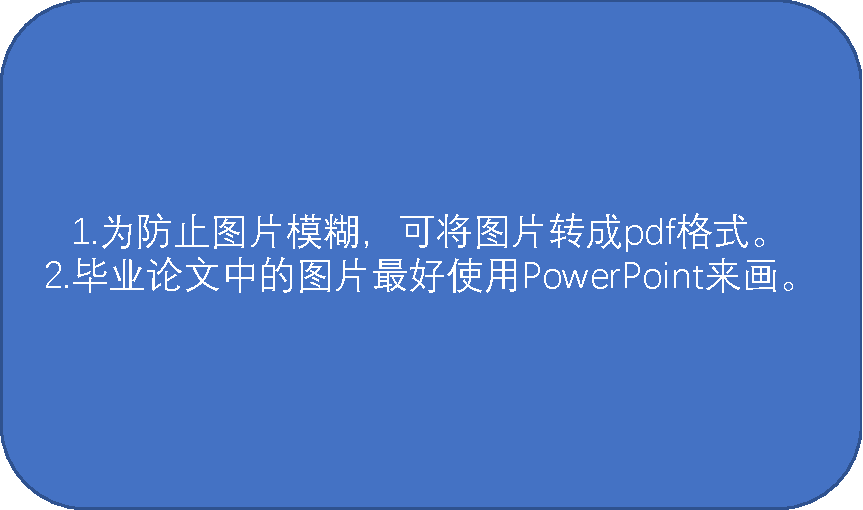
\includegraphics[width=\textwidth]{image/fig1.pdf}
%     \caption{代码示例的抽象语法树} 
%     \label{fig:fig1} 
% \end{figure}

\chapter{背景知识及相关技术}
本章节首先将会介绍与本文相关的研究工作,包括对于API文档的研究,对于Stack Overflow网站的研究,以及前人所做的在Stack Overflow上进行API知识抽取的研究。其次,本章节还会介绍本文使用到的一些方法与工具,如使用的信息抽取技术和自然语言处理技术等。

\section{API文档与Stack Overflow相关研究}
Robillard和Deline等人\cite{DBLP:journals/ese/RobillardD11}针对开发人员在学习API时遇到的困难进行了一系列经验研究。该研究设计了一系列对专业软件开发人员的调查和访谈,包括:

\begin{enumerate}
    \item 一项探索性的问卷调查,用于确定学习障碍的类别。
    \item 一组定性访谈调查,用于收集在工作中遇到的API学习障碍的具体场景。
    \item 一项后续问卷调查,用于确认该研究的结论并收集更多可能影响API学习障碍的额外因素。
\end{enumerate}

该研究在微软公司中展开,收集了440名专业软件开发者的调查结果。通过对调查结果进行分析,研究者发现开发人员在学习新API时面对的最大障碍来自于API文档的不足。而API文档的缺失体现在多个方面,如缺失与API的设计和原理相关的信息,缺少与使用场景相关的信息,缺少对API错误的处理指导以及缺少示例代码等等。

Mamykina等人\cite{DBLP:conf/chi/MamykinaMMHH11}对Stack Overflow进行了一系列的分析,她们通过将统计数据分析和用户访谈两种方法相结合\cite{DBLP:conf/chi/NamAA09},分析了Stack Overflow在软件工程领域取得成功的原因。该工作首先对整个Stack Overflow语料库进行分析,分别调查了回答时间、用户类型、不同问题类型的适用以及Stack Overflow这样的问答网站模型对其他领域是否可能存在拓展性,然后对网站的用户以及网站设计者进行了定性访谈研究。在软件工程领域,Stack Overflow取得了巨大的成功,网站上的问题回答率超过了90\%,远高于其他类似的问答网站,平均每个问题的回答耗时仅有11分钟。在用户访谈中,有许多用户认为Stack Overflow已经取代了搜索引擎,成为了他们解决编程问题的主要手段,同时还有一些用户认为自己在Stack Overflow网站上的高质量回答能为自己的简历增色不少。最后,Mamykina等人将Stack Overflow在软件工程领域的成功总结为精心设计的社区声誉系统,严格的社区准则,以及设计团队在自己设计的社区中积极地参与。

Treude等人\cite{DBLP:conf/icse/TreudeBS11}对Stack Overflow上提出的问题进行分类,并对不同类型问题的回答情况进行分析。该研究首先从Stack Overflow提供的API接口中获得了2010年11月1日至11月15日期间被提出的问题,并对这些问题进行定性分析和定量分析。通过对这些问题带有的标签以及问题标题与问题正文中出现的关键字进行分析,Treude等人将Stack Overflow上问题的标题分成10个类别,如表\ref{表2-1}所示。其中,出现频率最高的问题类型是how-to类型的问题。

\begin{table}[h]
    \centering
    \caption{Stack Overflow帖子标题分类\cite{DBLP:conf/icse/TreudeBS11}}
    \label{表2-1}
    \begin{tabular}{ll}
    \hline
    类别             & 具体描述                \\ \hline
    how-to         & 与寻求具体实现的指导相关的问题     \\
    discrepancy    & 作者想要得到解释的一些意外情况     \\
    environment    & 开发期间或部署后有关环境的问题     \\ 
    error          & 包含特定错误消息的问题         \\
    decision help  & 与意见征求相关的问题          \\
    conceptual     & 抽象且没有具体用例的问题        \\
    review         & 隐含或明确要求代码审查的问题      \\
    non-functional & 关于性能或内存使用等非功能性需求的问题 \\
    novice         & 明确指出提问者是一个新手        \\
    noise          & 与编程无关的问题          \\ \hline 
    \end{tabular}
\end{table}

在Treude等人的研究基础之上,Abdalkareem等人\cite{DBLP:journals/software/AbdalkareemSR17}针对开发人员如何使用Stack Overflow帮助自己完成编程任务继续进行了研究。该工作首先从GHTorrent数据集\cite{DBLP:conf/msr/Gousios13}中获取当前最流行的编程语言编写的Github项目,并从中筛选出较为活跃且成熟的项目。通过筛选设定条件为至少有100个pull request、至少有3个及以上开发人员以及过去的一年内至少有100次代码提交,Treude等人从数据集中找出那些符合要求的Github项目,再从这些项目的代码提交中找出那些提交日志中包含有Stack Overflow字样的,最后得到1780个符合条件的代码提交。通过对这些代码提交及其相关的Stack Overflow帖子进行人工统计,该工作将开发人员在Stack Overflow上寻求帮助的帖子分成了14个类别,如表\ref{表2-2}所示。

% Please add the following required packages to your document preamble:
% \usepackage{multirow}
\begin{table}[h]
    \centering
    \caption{Stack Overflow帖子知识需求分类\cite{DBLP:journals/software/AbdalkareemSR17}}
    \label{表2-2}
    \begin{tabular}{|c|c|c|}
    \hline
    主题                         & 副题          & 百分比   \\ \hline
    \multirow{9}{*}{运用知识}      & 编程语言        & 22.07 \\ \cline{2-3} 
                               & API使用       & 21    \\ \cline{2-3} 
                               & 配置管理        & 7.21  \\ \cline{2-3} 
                               & Web框架       & 6.51  \\ \cline{2-3} 
                               & Web浏览器      & 4.31  \\ \cline{2-3} 
                               & 开发工具        & 4.17  \\ \cline{2-3} 
                               & 实现问题        & 3.89  \\ \cline{2-3} 
                               & 数据库技术       & 2.83  \\ \cline{2-3} 
                               & 操作系统        & 2.4   \\ \hline
    \multicolumn{2}{|c|}{文档错误}               & 13.08 \\ \hline
    \multicolumn{2}{|c|}{Stack Overflow网站相关} & 3.18  \\ \hline
    \multicolumn{2}{|c|}{特性或系统改进}            & 1.77  \\ \hline
    \multicolumn{2}{|c|}{代码重用}               & 1.7   \\ \hline
    \multicolumn{2}{|c|}{其他}                 & 5.87  \\ \hline
    \end{tabular}
    \end{table}

该工作的统计数据表明,开发人员主要使用Stack Overflow来获取知识,常见的知识需求有编程语言特性、API使用、配置管理等,这部分Stack Overflow帖子占了数据集中的61.1\%。其次,开发人员还会使用Stack Overflow来记录自己在软件开发中遇到的错误,以及对于错误的解决方案等。这一部分类型的帖子在数据集中占有14.85\%。

从Abdalkareem等人的研究中我们不难得出结论,Stack Overflow的帖子中包含有许多有益于开发人员进行软件开发的知识,特别是与API相关的知识,这是本文选择Stack Overflow作为API知识抽取的语料库的原因。而通过Robillard等人的研究,我们可以得知现有的API文档无法满足程序员学习一个新API的需求。因此,许多开发者转而使用Stack Overflow作为学习新API知识的途径\cite{DBLP:conf/chi/MamykinaMMHH11}。在以上研究背景下,Stack Overflow具有作为API文档补充的巨大潜力,这也是所有基于Stack Overflow网站的API知识抽取研究工作提出的基础。

\section{API知识抽取相关研究}
为了从Stack Overflow网站上抽取出API知识并对API文档进行补充,国内外学者进行了许多研究工作。有部分学者使用了基于规则的抽取方式。Liu等人\cite{DBLP:conf/internetware/Liu0JMYZ18}采用了基于正则表达式和模式匹配的方法从多种属性的角度对Stack Overflow帖子中的知识进行分类,最后将帖子的知识分类结果用于设计一个Stack Overflow帖子的检索算法。Treude等人\cite{DBLP:conf/icse/TreudeBS11}的工作也基于规则匹配,他们设计了一些正则表达式来对Stack Overflow中的帖子标题和正文进行匹配,并对匹配得到的Stack Overflow帖子进行分类。这些工作有的是以较粗粒度的帖子作为对象的,也有的是以较为细粒度的句子级文本作为操作对象的。

此外,还有许多学者采用了基于机器学习的抽取方式。Treude等人\cite{DBLP:conf/icse/TreudeR16}在之前工作的基础上,提出了一种称为SISE的API知识抽取方法。如表\ref{表2-3}所示,SISE从了Stack Overflow帖子抽取出大量信息作为句子特征,包括句子文本本身,句子的语言模式,句子的归属问题,归属回答,帖子的作者,句子中的词性标签以及该句子与相应API文档的句子相似度等,并用这些句子特征训练了一个分类模型,用于从Stack Overflow帖子中抽取出带有API观点的句子。该工作的研究者人工标注了1574个来自Stack Overflow中的句子作为开发集,并通过实验证明了SISE在开发集上表现良好,能够达到0.64的准确率和0.7的覆盖率。

\begin{table}[h]
    \centering
    \caption{SISE方法中的句子特征\cite{DBLP:conf/icse/TreudeR16}}
    \label{表2-3}
    \begin{tabular}{ll}
        \hline
        \# & 特征                            \\ \hline
        1  & 句子与API文档中最相似句子之间的余弦相似度        \\
        2  & 句子与API文档中所有句子之间的平均余弦相似度       \\
        3  & 问题的用户接受率                      \\
        4  & 回答的得分                         \\
        5  & 回答的年龄                         \\
        6  & 回答耗时                          \\
        7  & 问题得分                          \\
        8  & 问题收藏数                         \\
        9  & 提问者的声誉                        \\
        10 & 问题的浏览次数                       \\
        11 & 句子中放在动词前的第三人称单数现在进行时形式的名词数量   \\
        12 & 问题的年龄                         \\
        13 & 句子是否以放在动词前的第三人称单数现在进行时形式的名词开头 \\
        14 & 句子包含的词语个数                     \\
        15 & 句子中API提及出现的位置                 \\
        16 & 句子中API提及出现的次数                 \\
        17 & 回答的得分                         \\
        18 & 回答的长度                         \\
        19 & 句子中名词的数量                      \\
        20 & 句子是否以名词开头                     \\
        21 & 句子中代码片段的字符数                   \\
        22 & 句子中单词“be”的出现次数                \\ \hline
    \end{tabular}
\end{table}

Uddin等人\cite{DBLP:journals/tse/UddinK21}针对Stack Overflow上讨论API的句子进一步拓展了前人关于软件工程领域情感分析方面的研究。在之前的研究中,有许多学者针对软件工程领域的文本情感分析进行了许多工作,如对Github上的评论进行情感分析\cite{DBLP:conf/kbse/UddinK17}\cite{DBLP:conf/msr/PleteaVS14}\cite{DBLP:conf/msr/GuzmanAL14}\cite{DBLP:conf/sigsoft/GuzmanB13},以及对传统的情感分析工具在软件工程领域的表现进行了实验对比\cite{DBLP:conf/icsm/JongelingDS15}。由于传统的情感分析工具在软件工程领域表现不佳,Uddin等人基于Hu和Liu等人\cite{DBLP:conf/kdd/HuL04}提出的主导情绪取向算法和Thelwall等人\cite{DBLP:journals/jasis/ThelwallBPCK10}实现的情感分析工具SentiStrength进行了改进,实现了更贴近软件工程领域需求的情感分析算法OpinerDSOSenti。同时,他们还设计了一系列调查,用于了解开发人员更喜欢在论坛上讨论关于API的哪些方面,并通过分析来自178名专业软件开发人员的回答将关于API的意见分成了11类,如表\ref{表2-4}所示。最后,Uddin等人使用OpinerDSOSenti算法在随机采样得到的1338个Stack Overflow帖子中对所有句子进行情感分析,并将抽取得到的带有情感倾向的句子分类到提出的11中类别中。该工作的抽取结果与人工标注的结果对比表明,OpinerDSOSenti在抽取带有情感倾向的句子方面准确率较高,达到了0.778,而在分类准确率上表现较为一般,仅有0.502的正确率。较低的分类准确率可能是由于作者设计的知识分类类型较多,模型不能很好地区分不同类型知识之间的特征。

\begin{table}[h]
    \centering
    \caption{Opiner工具对API意见的分类\cite{DBLP:journals/tse/UddinK21}}
    \label{表2-4}
    \begin{tabular}{|l|l|}
        \hline
        类别        & 定义                                                                      \\ \hline
        性能        & 与一个API的性能相关的观点                                                          \\ \hline
        可用性       & 一个API是否是好用的                                                             \\ \hline
        安全        & \begin{tabular}[c]{@{}l@{}}与安全原则、安全漏洞的影响以及对API最佳安全实现\\ 的观点\end{tabular} \\ \hline
        文档        & 该API在各种开发资源中是如何被记录的                                                     \\ \hline
        兼容性       & 该API在一个给定的框架中是如何工作的                                                     \\ \hline
        可移植性      & 该API是否能在不同的操作系统下工作                                                      \\ \hline
        社区        & 使用和开发该API的开发者是否能快速响应                                                    \\ \hline
        合法性       & 关于一个API的许可问题的观点                                                         \\ \hline
        漏洞        & \begin{tabular}[c]{@{}l@{}}关于该API的某个特定漏洞的存在、扩散以及修复的\\ 意见\end{tabular}   \\ \hline
        其他通用API特性 & 其他关于该API的特性或用法的意见                                                       \\ \hline
        情绪表达      & 只有情绪表达,而不涉及具体方面的观点                                                      \\ \hline
        \end{tabular}
        \end{table}

\section{基于自举(Bootstrapping)思想的信息抽取技术}
从知识图谱这一学科建立以来,知识抽取就一直是该领域研究的一个重要方向。在机器学习技术非常成熟的今天,许多学者更倾向于结合最新的深度学习技术来取得更好的知识抽取效果。然而,在工业界,基于自举思想的自举抽取法作为一种老而弥坚的知识抽取方法仍然能在较低的技术门槛下取得非常好的效果。该方法最早由Brin在1998年提出\cite{DBLP:conf/webdb/Brin98},这是一种被命名为DIPRE(Dual Iterative Pattern Expansion)的半监督的结构化关系抽取方法,能够通过在非常少的实例中学习种子模板,然后在大量非结构化文本中使用这些种子模板抽取出新的实例,同时在抽取出的新实例中学习得到新的模板,并继续使用这些新的模板抽取实例。DIPRE方法的工作流程如图2-1所示。

\begin{figure}[htb]
    \centering
    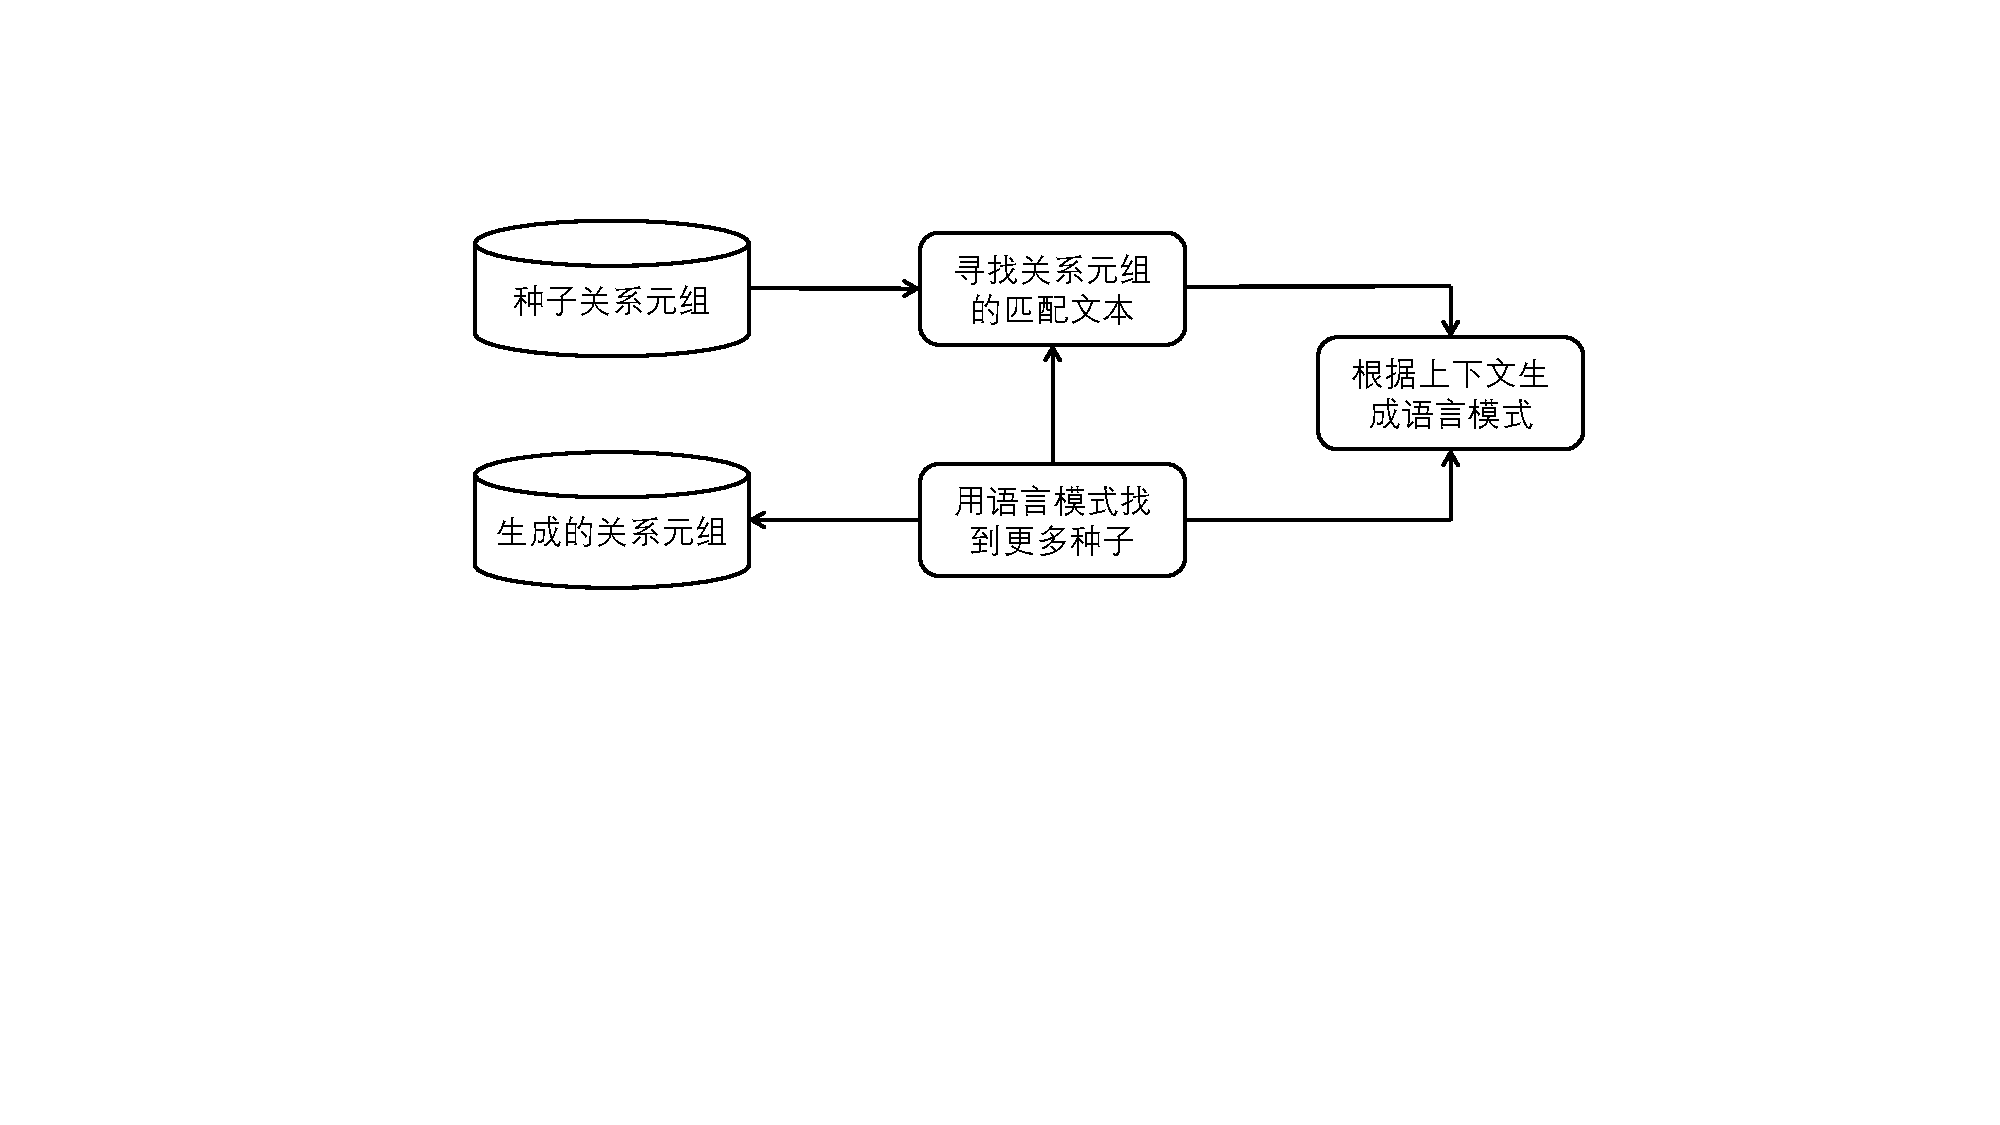
\includegraphics[width=\textwidth]{image/DIPRE.pdf}
    \caption{DIPRE方法工作流程\cite{DBLP:conf/webdb/Brin98}} 
    \label{fig:fig1} 
\end{figure}

Agichtein\cite{DBLP:conf/sigmod/AgichteinGV01}在Brin的基础之上对方法进行了改进,设计实现了Snowball信息抽取系统。与DIPRE相比,由Snowball抽取出来的模板包含了来自种子的命名实体标签,并且设计了一种用于在抽取的过程中评估每次迭代生成的模板和种子的策略,在迭代抽取信息的过程中只保留那些被认为是可靠的种子和模板。通过这些优化设计,Snowball系统取得了比DIPRE更好的效果,在Agichtein设计的对比实验中,Snowball系统和DIPRE系统得到了相近的精确率,但Snowball的召回率更高。

在这之后,还有许多学者基于DIPRE方法继续进行优化,如Carlson等人\cite{DBLP:conf/aaai/CarlsonBKSHM10}设计了NELL(Never-Endding Language Learner)知识抽取系统,只需提供一个种子模式,就能在大规模的Web文本上迭代地抽取知识,并通过对抽取出来的文本知识打分来提高抽取的准确率。

本文也是基于自举思想实现的知识抽取方法,针对软件工程领域设计了特定的知识概念模型,并针对API知识这一抽取目标设计了合理的知识抽取方法。

\section{自然语言处理工具}
本小节将会介绍本文使用到的与自然语言处理的相关工具,包括自然语言解析工具spaCy,以及它提供的数个模块,还有Facebook公司提出的文本分类算法fastText,以及该算法的封装库。
\subsection{spaCy及其原理}
spaCy\footnote{https://spacy.io/}是一个用于自然语言处理的Python开源模块,可以用于构建处理和理解大量文本的程序。得益于在许多相关模块使用Cython(一种Python的C语言拓展,旨在让Python程序的性能够接近C语言程序)进行优化,spaCy的性能非常强大,与科研工作常用的Python自然语言处理库NLTK相比,它的解析速度更快,且为CPU进行了针对性优化,这让spaCy在没有GPU的环境下也能很好地工作。

spaCy提供了非常简便的调用方式来对自然语言文本进行处理,包括文本清洗、分词、分句、命名实体识别、词干化、词性标注和依赖解析功能等,这些都基于已经训练好的机器学习和深度学习模型(如BERT等)实现。spaCy的可拓展性非常强,用户可以根据自己的需要对整个文本处理流程进行定制,增加、修改自己所需要使用的管道组件,并移除自己所没有使用到的文本处理模块。spaCy的高可拓展性进一步提高了它的性能。

spaCy中的Tokenizer模块用于支持分词、分句功能,它由前缀模式、中缀模式、后缀模式和特殊规则组成。在文本处理的过程中,spaCy先将文本进行简单的空格分词,Tokenizer再从左向右依次处理词语,检查词语是否匹配特殊规则、或者是前中后缀中的一种,再根据这些模式进行分词。本文中对spaCy的优化主要是对Tokenizer模块的修改,让spaCy的分句、分词更加契合Stack Overflow网站上的讨论文本,如适应API提及句子的分句、适应对特殊符号的分词等,提高数据的整体质量。

spaCy还提供了Matcher模块,允许用户制定规则进行文本匹配,匹配的规则可以是基于文本,基于词性标签,或者基于词法属性。与文本匹配常用的正则表达式相比,spaCy的Matcher模块不仅能找到符合规则的文本,还能对文本中的单词进行访问,获得其词性等属性,或者在单词级别对文本进行修改。本文使用到了Matcher模块用于从一个描述了API知识的句子中抽取出代表该种API知识表达方式的语言模式,并用这些模式在语料库中寻找相似的句子。

除了Matcher模块之外,spaCy还为用户提供了PhraseMatcher模块。PhraseMatcher模块提供了同时检索多个词语的方法。通过将需要检索的词汇表添加到一个PhraseMatcher中,就能实现快速判断一个句子是否包含词汇表中的所有单词。这种判断方式比常规的字符串匹配更为高效,故本文使用了这一模块作为从语料库中匹配API知识的方式,从而提高方法流程的整体效率。

\subsection{fastText}
fastText\footnote{https://fasttext.cc/}是由Facebook公司开源的一个用于文本分类的Python开源模块,通常用于带监督的文本分类问题。fastText算法在学术上并没有非常显著的创新,但它结合了在自然语言处理与机器学习领域中已有的优秀算法,这让它在拥有与基于深度学习算法的文本分类器不相上下的高精度的同时还具有更快的模型训练速度以及预测速度。

在机器学习技术已经发展得非常成熟的今天,基于神经网络的文本分类技术在实践中表现优异,但它们在训练和测试时往往较慢,这一特点限制了基于神经网络的文本分类技术在大型文本数据集上的运用。同时,过去的线性文本分类技术虽然已提出多年,但在选择合适的句子特征作为输入时,它的表现并不比基于神经网络的分类器差。

因此,Joulin等人提出了fastText方法\cite{DBLP:conf/eacl/GraveMJB17},将早期的线性文本分类技术进行优化,大大提高了它在大型文本数据集上运行的效率。fastText算法的模型结构如图\ref{图2-1}所示。fastText算法使用了词袋特征以及n-gram特征来表征一个句子,通过线性变换来将这些句子特征映射到模型架构的中间层中,再使用一个基于哈夫曼编码的层次softmax分类器将句子分类到特定的标签中。由于线性文本分类器在特征和类别之间不共享参数,这可能会影响到它在大型文本数据集上的泛化表现。为了解决这一问题,Joulin等人将线性分类器分解为低秩矩阵。

\begin{figure}[htb]
    \centering
    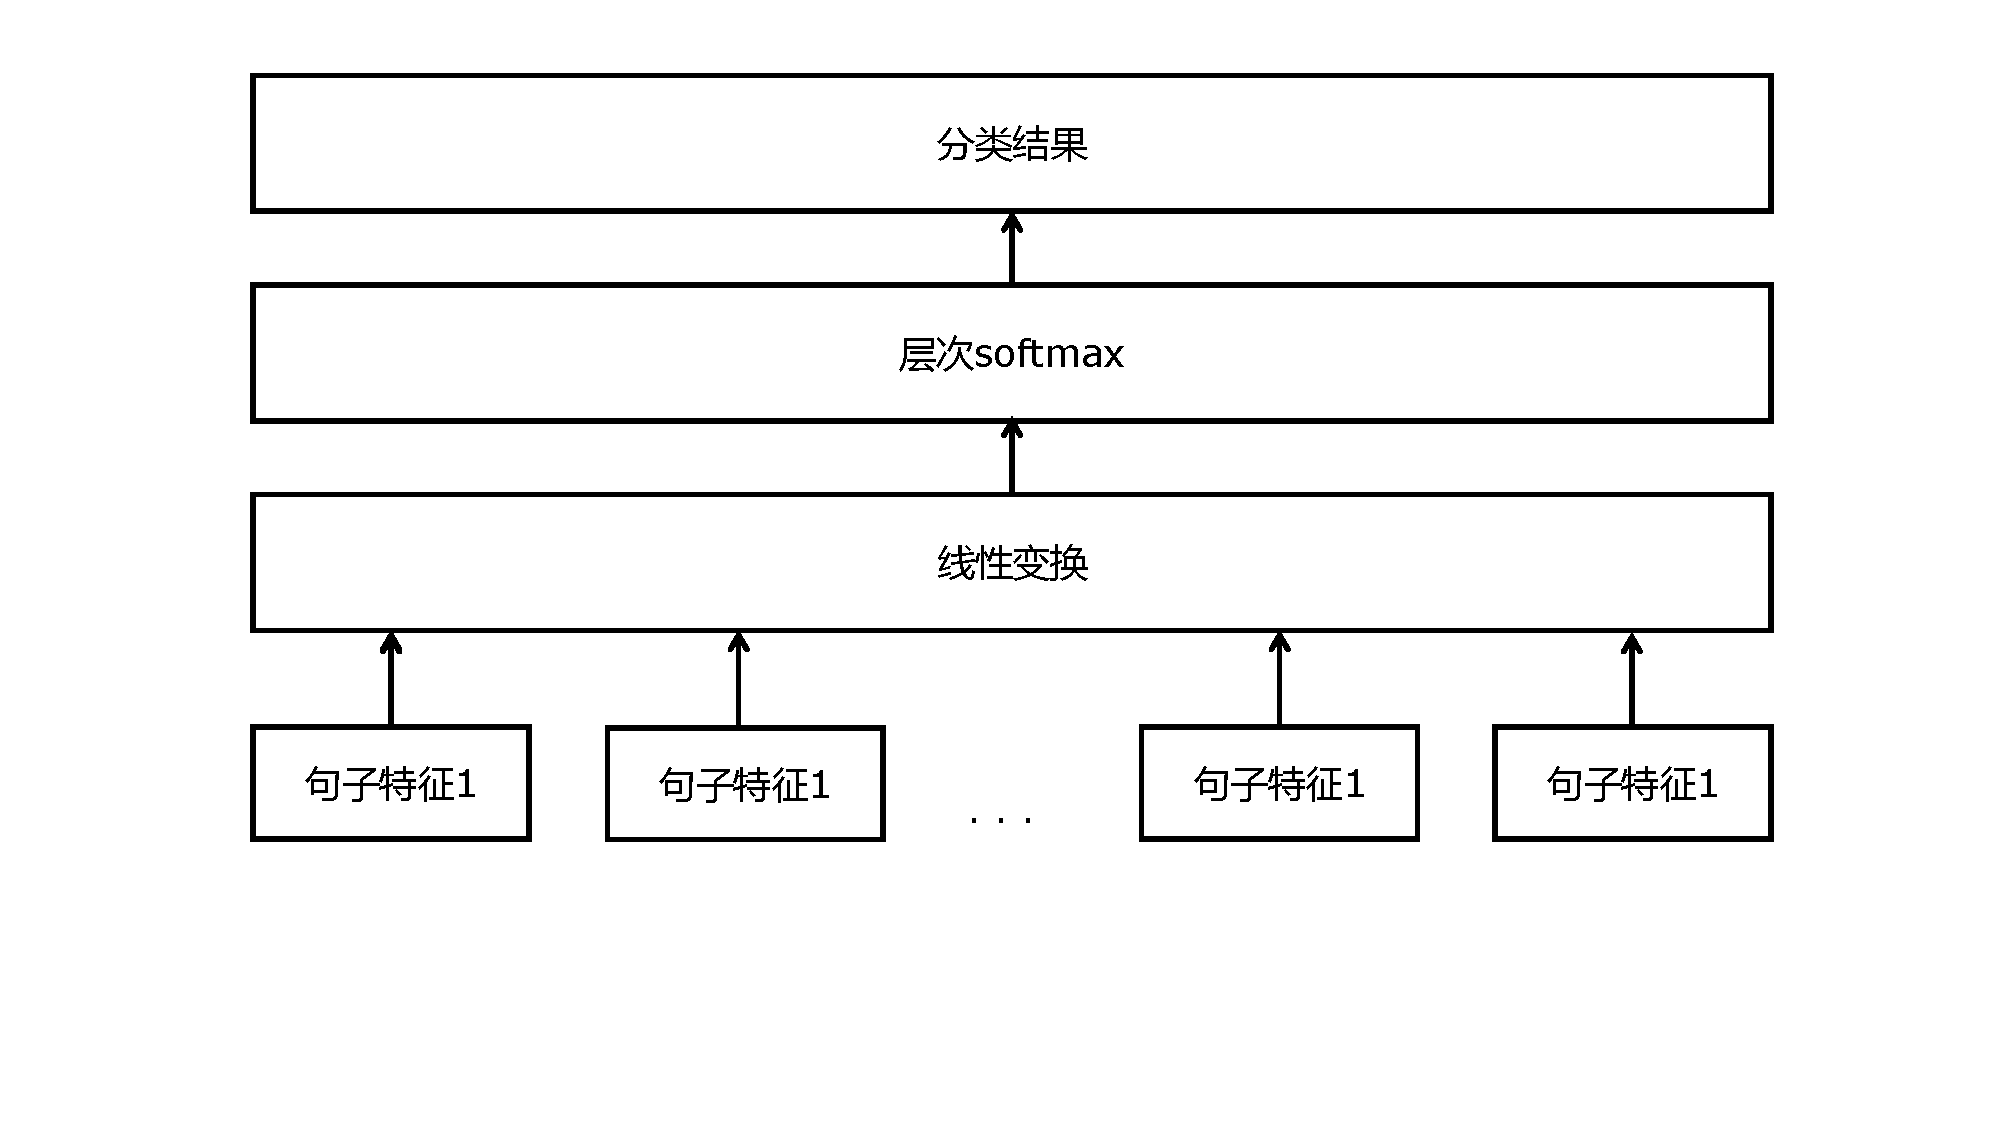
\includegraphics[width=\textwidth]{image/fast-text.pdf}
    \caption{fastText模型结构\cite{DBLP:conf/eacl/GraveMJB17}} 
    \label{图2-1} 
\end{figure}

当分类的类别过多时,标准的归一化softmax效率较低,时间复杂度是O(kh),其中k是类别的数量,h是文本表示的维度。为了提高速度,Joulin等人通过使用基于哈夫曼编码树的分层softmax,使得计算一个句子所属类别的时间复杂度降低到O(hlog2(k))。这让fastText在计算一个句子分类到某个标签的概率的速度大大地提高了。

Facebook公司开源的Python第三方库 fastText 提供了fastText算法直观易用的调用方式,让用户不需要预训练词向量,只需提供预标注的训练数据就可以在极短的时间内训练出一个高精度的文本分类器。与传统的基于神经网络的文本分类器相比,fastText的训练速度要快上若干个数量级。在标准的多核CPU上,fastText能够在10分钟之内训练10亿个词级别的语料库的词向量,并且能够在1分钟内将具有30万种类别的50多万条句子完成分类。

本文使用了fastText库,预标注并训练出一个文本分类器用于识别出Stack Overflow帖子中的API描述性知识句子,通过这种方式来生成一个高质量的语料库,保证了本方法抽取出来的知识的质量。

\section{本章小结}
本章主要介绍了与API文档,Stack Overflow和API知识抽取技术的相关研究,以及本文所使用到的相关技术。本章首先介绍了与API文档和Stack Overflow网站相关的研究,说明了对于软件开发人员来说API文档并不足以满足日常开发需求,而Stack Overflow网站上包含有大量与API相关的众包知识能够作为API文档的补充。之后介绍了其他学者基于Stack Overflow网站进行的API知识抽取工作,包括基于规则和基于机器学习的方法。然后介绍了基于自举思想的信息抽取技术,以及它的衍生工作。最后,本章还介绍了本方法中使用到的一些工具,包括自然语言处理工具spaCy和文本分类器fastText。


\chapter{方法概述}
本文提出了一种从软件开发问答网站Stack Overflow中抽取出API描述性知识的方法。本章首先会详细介绍本文定义的API描述性知识概念模型,并给出一个运行示例用于展示本文方法流程。然后,本章会对API描述性知识抽取方法中的每个步骤进行详细说明。本抽取方法的流程概览如图\ref{图3-1}所示:

\begin{figure}[htb]
    \centering
    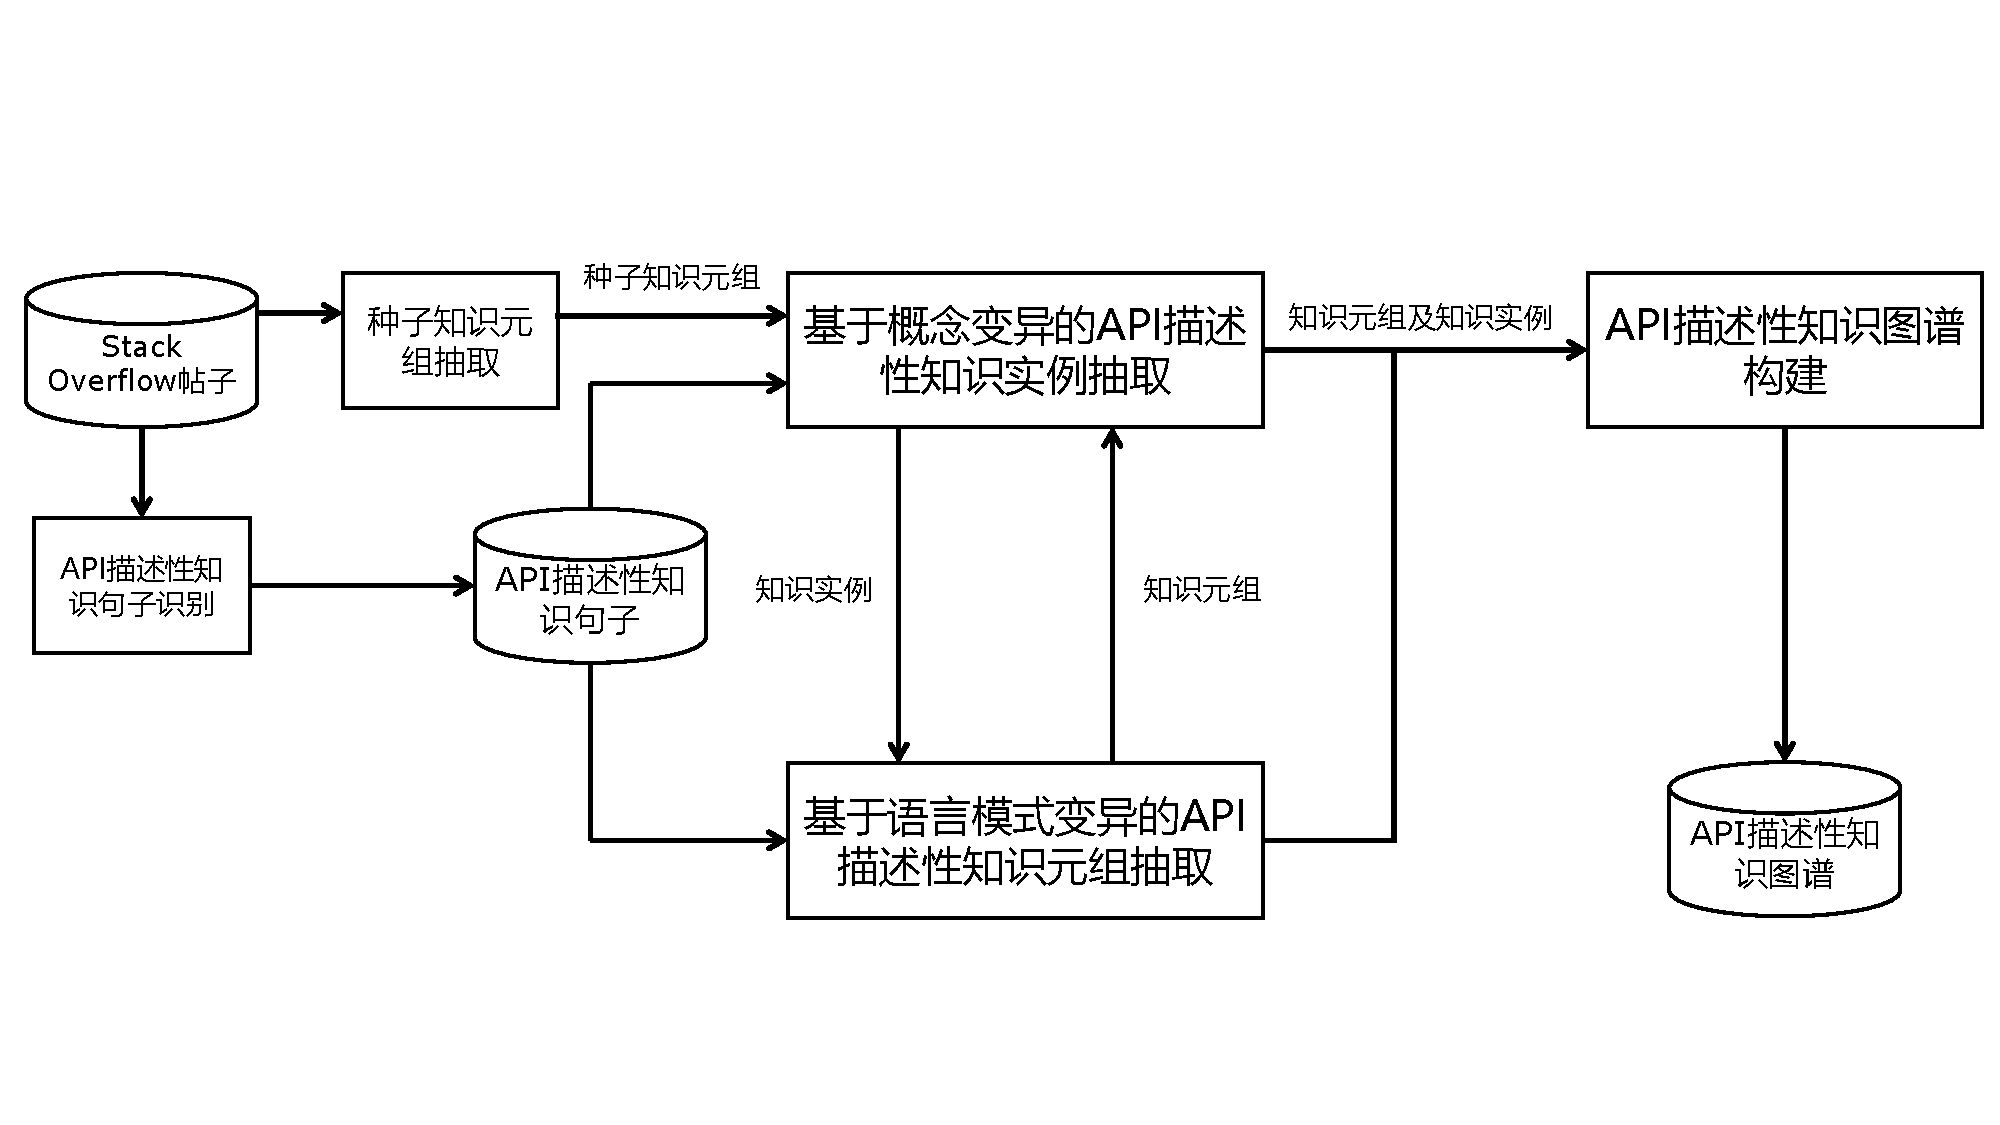
\includegraphics[width=\textwidth]{image/overview.pdf}
    \caption{API描述性知识抽取流程概览} 
    \label{图3-1} 
\end{figure}

本文提出的方法可以分为五个步骤:
\begin{enumerate}
    \item API描述性知识句子识别。该步骤从Stack Overflow网站的数据中抽取过滤出用于抽取API描述性知识的语料库,详细内容在章节3.3中说明。该步骤的流程如下:
    \begin{enumerate}
        \item Stack Overflow帖子获取。从完整的Stack Overflow网站数据库中设置一定的条件进行筛选,得到用于生成语料库的帖子集合。
        \item API描述性知识句子候选抽取。使用优化过的spaCy工具对上一步中得到的帖子的文本进行分句,并进行一系列基于正则规则的过滤,得到包含有API提及的句子作为候选。
        \item API描述性知识句子分类。使用一个训练好的fastText文本分类器,对上一步中得到的带有API提及的句子进行分类,将分类出来的API描述性知识句子作为用于抽取API描述性知识的语料库。
    \end{enumerate}
    \item 种子知识元组抽取。该步骤根据本方法指定的规则,从API描述性知识句子中抽取出知识元组,作为下一步骤的输入。详细生成规则在章节3.4中介绍。
    \item 基于概念变异的API描述性知识实例抽取。该步骤根据给定的API描述性知识元组进行知识抽取,详细的介绍在章节3.5中。本步骤的流程如下:
    \begin{enumerate}
        \item 知识元组过滤。对于给定的API描述性知识元组,本方法设定了一系列规则对其进行过滤,筛选掉其中质量不高的知识元组。
        \item 知识元组变异。对上一步中过滤后的知识元组,将它们根据定义好的一系列变异方式进行修改变异,得到更多的知识元组,这些变异得到的知识元组是潜在的API描述性知识。
        \item 知识元组匹配。使用种子API描述性知识元组和变异得到的API描述性知识元组在语料库中进行匹配,获得API描述性知识实例句子。    
    \end{enumerate}
    \item 基于语言模式变异的API描述性知识元组抽取。该步骤根据给定的API描述性知识实例句子进行知识抽取,得到更多API描述性知识元组。详细流程见章节3.6。其子步骤如下:
    \begin{enumerate}
        \item 语言模式抽取。从上一步中匹配得到的API描述性知识实例句子中总结出这个句子的语言模式,这个语言模式可能代表了人们常用于描述这种类型的知识的习惯用语。
        \item 语言模式变异。得到语言模式后,通过设定好的规则对其进行泛化修改,得到若干变异后的语言模式。
        \item 语言模式匹配。使用上一步中得到的变异语言模式在语料库中进行匹配,找到那些符合语言模式的句子,这些句子也是API描述性知识实例句子。从这些句子中可以总结出新的API描述性知识元组。
    \end{enumerate}
    步骤3和步骤4的执行逻辑如算法1所示。步骤3输出的API描述性知识实例就是步骤4的输入数据,而步骤4输出的API描述性知识元组则可以作为步骤3的输入数据。通过迭代地执行步骤3和步骤4,本方法可以从语料库中不断地抽取出API描述性知识。迭代抽取的程序逻辑如算法2所示。
    \item API描述性知识图谱构建。将上述步骤中抽取得到的API描述性知识以及API描述性知识实例句子以图谱节点的形式保存到知识图谱中,并为它们构建节点之间的关系。详细的知识图谱设计见章节3.7。
\end{enumerate}

\floatname{algorithm}{算法}  
\renewcommand{\algorithmicrequire}{\textbf{输入:}}  
\renewcommand{\algorithmicensure}{\textbf{输出:}}  
\begin{algorithm}  
    \caption{API描述性知识抽取的单步流程} 
    \begin{algorithmic}[1] %每行显示行号  
        \Require $currentSeedList$种子API描述性知识元组,$sentenceList$语料库,$result$上一轮迭代抽取得到的结果
        \Ensure $result$新一轮知识抽取得到的结果
        \Function{runForOneStep}{$currentSeedList, sentenceList, result$}  
            \State 过滤currentSeedList和sentenceList
            \State currentSeedList \gets currentSeedList变异得到的知识元组
            \State InstanceList \gets currentSeedList和sentenceList匹配得到的知识实例
            \State patternList \gets 从InstanceList中抽取并变异得到的语言模式
            \State patternInstancePair \gets PatternList和sentenceList匹配得到的知识实例
            \State newSeedList \gets 从patternInstancePair中抽取出的知识元组
            \State 将上述结果保存到result中
            \State \Return{$result$}
        \EndFunction  
    \end{algorithmic}  
\end{algorithm} 

\floatname{algorithm}{算法}  
\renewcommand{\algorithmicrequire}{\textbf{输入:}}  
\renewcommand{\algorithmicensure}{\textbf{输出:}}  
\begin{algorithm}  
    \caption{API描述性知识抽取的总体流程}  
    \begin{algorithmic}[1] %每行显示行号  
        \Require $seedList$种子API描述性知识元组,$sentenceList$语料库,$maxStep$最大迭代次数,$saveByStep$每多少步保存一次  
        \Ensure $result$保存了API描述性知识抽取结果的Snowball对象  
        \Function {run}{$seedList, sentenceList, maxStep, saveByStep$}  
            \State result \gets []
            \For{i = 1 \to maxStep+1}
                \If {i == 1}
                    \State currentSeedList \gets seedList
                \Else
                    \State currentSeedList \gets 上一轮抽取得到的API描述性知识元组
                \EndIf
                \State result \gets \Call{runForOneStep}{$currentSeedList, sentenceList, result$}
                \If {i \% saveByStep == 0}
                    \State 将result保存到本地
                \EndIf
            \EndFor
            \State 将result保存到本地
            \State \Return{$result$}  
        \EndFunction  
    \end{algorithmic}  
\end{algorithm} 

\section{API描述性知识概念模型}
通过观察Stack Overflow中与API相关的讨论帖子,以及对帖子中带有API知识的句子进行分析,本文定义了一个概念模型,用于描述本文所定义的API描述性知识及其相关概念
。
图\ref{图3-2}为本文定义的API描述性知识概念模型。本文抽取得到的API描述性知识来自于Stack Overflow中与API相关的讨论。其中,API相关讨论包含了API相关的问题以及这些问题的回答,而与API相关的问题回答为本文提供了API描述性知识句子。API描述性知识句子是一个包含了与API功能、API特性或API表现相关的知识的句子。本方法能够从一个API描述性句子中抽象出一个API描述性知识元组,这个知识元组由若干个API知识元素组成。API知识元素分为4种类别,分别是API元素,动作,目标对象以及特性。除了API元素以外,其他三种API知识元素的分类依据是词语的词性,本文将动词词性的知识元素视为动作类型,将名词词性的知识元素分为目标对象类型,将形容词与副词词性的知识元素分为特性类型。

\begin{figure}[htb]
    \centering
    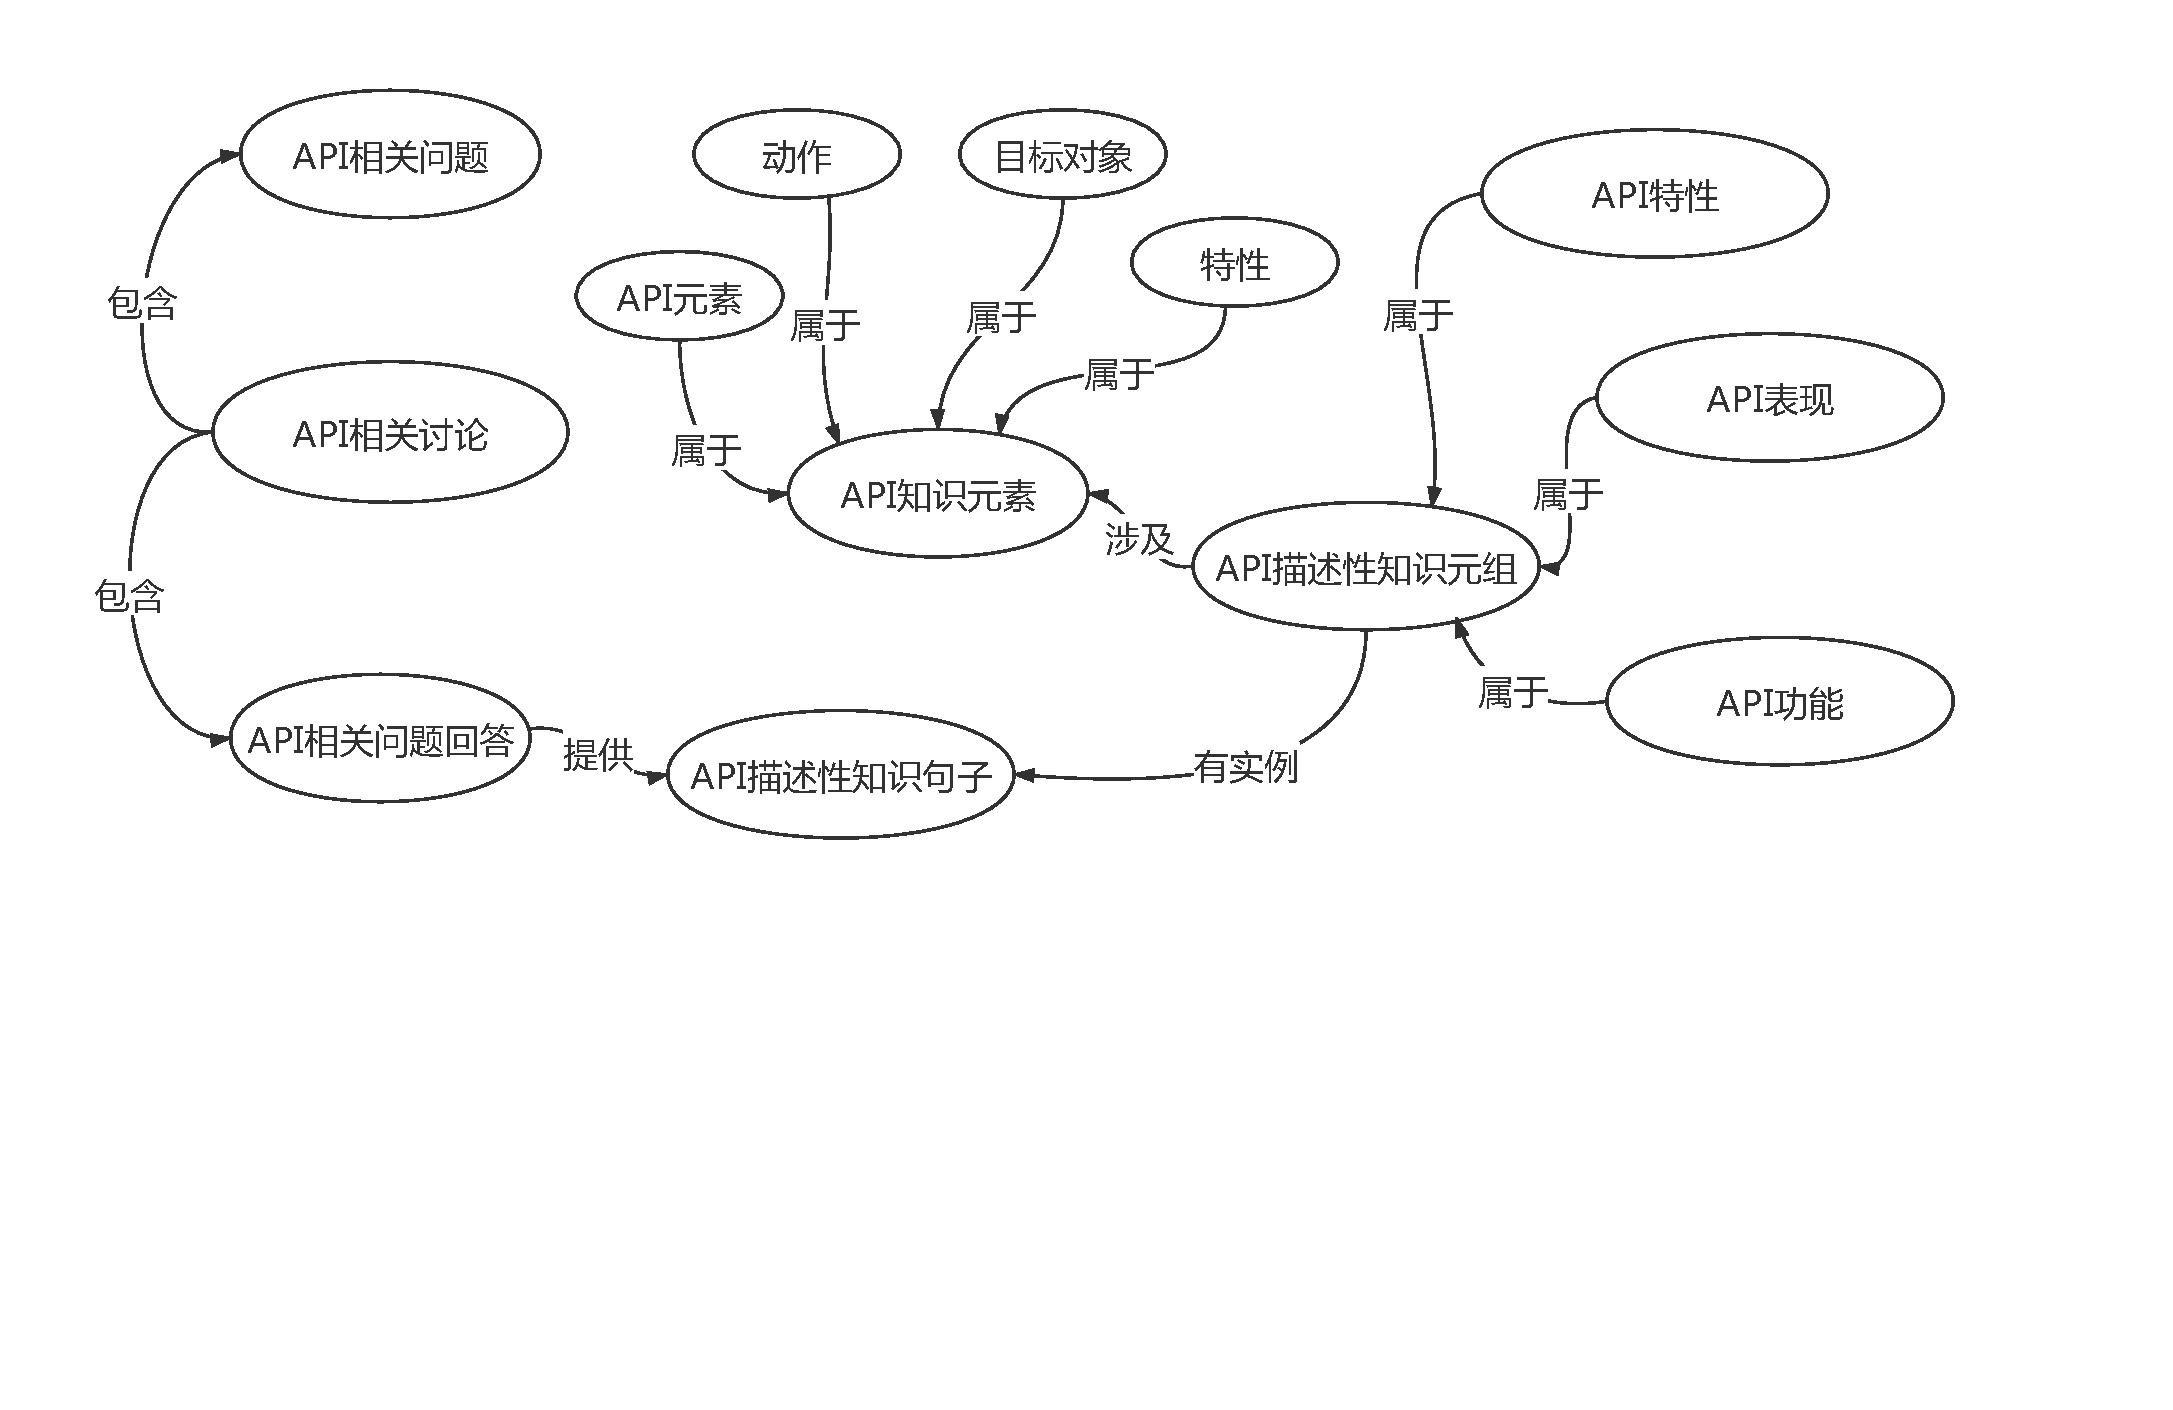
\includegraphics[width=\textwidth]{image/structure.pdf}
    \caption{API描述性知识相关概念模型} 
    \label{图3-2} 
\end{figure}

举例来说,一个API描述性知识句子:“The StringBuffer class is thread-safe.”,从这个句子中可以抽象出一个API描述性知识元组:<API:[StringBuffer], Characteristic:[thread-safe]>,它包含一个指明当前知识所属API的API元素,以及一个特性类型的API知识元素Characteristic。

根据一个API描述性知识元组所包含的API知识元素类型不同,API描述性知识也被分为三种类型,分别是API特性、API表现以及API功能。当一个知识元组仅包含特性类型的知识元素时,它会被分类为描述API特性的知识,如上一段话中所举的例子,就是一个API特性知识;当一个知识元组包含了动作和目标对象类型的知识元素时,它将被视为一个API功能类型的API描述性知识。举例而言,从句子“removeFirst() : Remove the first element in the list.”中,可以抽象出一个知识元组:<API:[removeFirst()], Action:[remove],Object:[the first element]>,这个知识元组是被分类为API功能的知识;最后,当一个知识元组包含了动作和特性知识元素时,它会被分类成描述API表现的知识,比如从句子“You can also use the javax.swing.Timer to hide this popup automatically.”中,可以抽象出一个API表现类型的知识元组<API:[javax.swing.Timer],Action:[hide],Characteristic:[automatically]>,它会被分类为API特性类型。

\section{运行示例}
本小节会使用一个API描述性知识元组作为示例,展示出本方法抽取流程的一次迭代过程,以及抽取过程中各步骤的输出。

本文首先在语料库中人工抽取出高质量的API描述性知识元组作为迭代的种子知识元组,例如,从句子“The StringBuffer class is thread-safe”中提取出知识元组<API:[StringBuffer], Characteristic:[thread-safe]>。

在每一轮迭代的开始,首先对种子进行过滤,过滤掉质量较低的种子,防止错误传递。

对剩下的高质量种子,本方法使用预设的规则对这些种子知识元组进行修改,得到一系列变异过的知识元组。例如,从知识元组<StringBuffer, thread-safe>可以变异得到一个新的知识元组<StringBuffer, synchroinzed>。这些变异得到的API描述性知识元组是潜在的可能可以从语料库中被抽取出来的API描述性知识实例的抽象表示。

变异完成后,使用这些知识元组(包括种子知识元组和变异知识元组)在语料库中进行匹配,以找到这些知识元组的实例句子。在本例子中,语料库中的句子“Each method in StringBuffer is synchronized”可以作为变异得到的知识元组<StringBuffer, synchronized>的一个实例被抽取出来。这个被抽取出来的API描述性知识实例可以用于生成这种知识的语言模式。在本示例中,上述实例包含的元素会被标注出来,进而得到“Each method in (API)[StringBuffer] is (Characteristic)[synchronized]”。

下一步是基于语言模式的变异。对上述匹配得到的API描述性知识实例,本方法抽取出其中的语言模式,并对模式中的原知识元组中的元素所在位置的词语进行变异,从而从一个已有的知识实例中生成若干可能可以代表这一知识形式的语言模式。例如,API描述性知识实例“Each method in (API)[StringBuffer] is (Characteristic)[synchronized]”可以变异得到新的句子模式“Each method in (API)[StringBuffer] is (Characteristic)[ADJ]”。其中,“[ADJ]”代表了一个词语通配符,表示可以匹配上任何一个形容词性或副词词性的词语及短语。语言模式使用新的句子模式在语料库中进行匹配,找到匹配的实例句子后,可以从中抽取出新的API描述性知识元组。例如,使用上述句子模式,可以匹配出句子“Each method in StringBuffer is ineffective”,从中可以提取出新的API描述性知识元组<API:[StringBuffer], Characteristic:[ineffective]>。

这样就完成了本方法的一轮迭代抽取流程。而在下一轮的知识抽取中,新的API描述性知识元组<API:[StringBuffer], Characteristic:[ineffective] >会作为下一轮迭代抽取的种子,继续进行变异、匹配。


\section{API描述性知识句子识别}
在执行API描述性知识的抽取流程之前,本方法需要准备好用于抽取知识的语料库,以及作为抽取流程起点的种子知识元组。本节将会介绍本文是如何从Stack Overflow中识别出API描述性知识句子的。图\ref{图3-3}展示了一个Stack Overflow与API讨论相关的问答帖子,以及在回答中包含的一个API描述性句子。

\begin{figure}[htb]
    \centering
    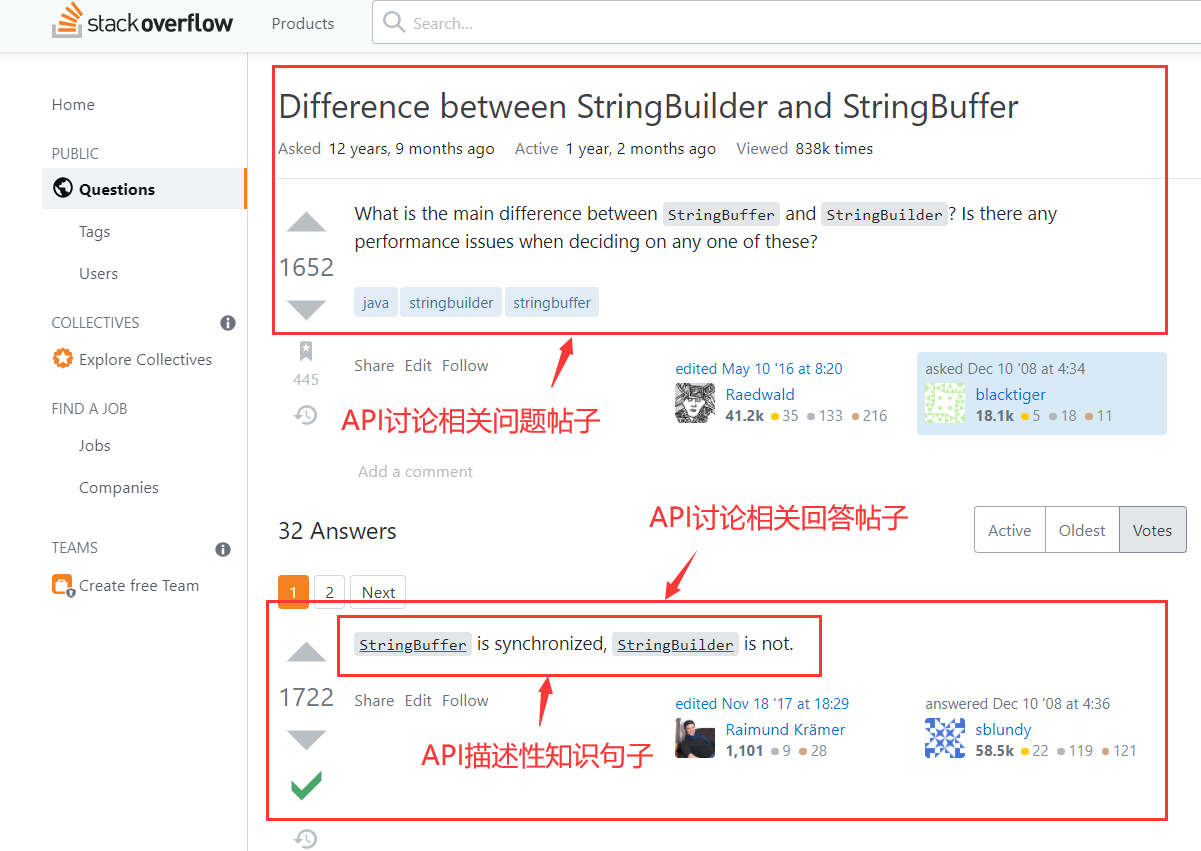
\includegraphics[width=\textwidth]{image/so.png}
    \caption{Stack Overflow中的API描述性知识句子示例} 
    \label{图3-3} 
\end{figure}

\subsection{Stack Overflow帖子获取}
本工作中进行API描述性知识抽取的语料库来自Stack Overflow。Stack Overflow官方会定期将论坛中的所有帖子数据打包,并公开发布以供学者研究(本文所使用的帖子数据是Stack Overflow官方于2021年3月发布的数据)。当然,Stack Overflow上的帖子数量过于庞大,而且并不是每一个帖子都具有被抽取的价值。因此,本方法设定了以下条件作为筛选,从Stack Overflow的所有帖子中找到符合条件的帖子作为抽取API描述性知识句子的来源:

\begin{itemize}
    \item 帖子是一个回答类型的帖子。通常,对于一个API的讨论更有可能出现在一个问题的回答中。
    \item 帖子的得分大于0。如果帖子的得分大于0,那就说明至少有一位其他用户对这篇回答持支持态度,也就意味着该回答有被抽取的价值。
    \item 帖子的标签列表中包含<java>标签。在今天,Java仍然是世界上应用最广泛的编程语言之一,开发者对Java语言相关的API知识需求很高,且Java标签是Stack Overflow上最热门的标签之一,这保证了本文语料库的规模。
\end{itemize}

\subsection{API描述性知识句子候选抽取}
对于一个含有API描述性知识的句子而言,这个句子中既有可能直接出现一个API的提及,也可能该API是在上下文中已经出现过,而在该句子中只有代词指代。显然,包含API描述性知识的句子并不一定包含API提及,但包含API提及的句子更有可能是一个包含API描述性知识的句子。因此,对于上一步中筛选得到的帖子中的所有句子,可以在其中筛选出带有API提及的句子作为候选,这些句子更有可能抽取出API描述性知识。

在筛选出帖子后,本方法对帖子进行分句。分句时,软件工程领域相关文本的一些特点可能会对分句产生影响,经过人工的观察,我们发现常见的会对文本分句造成影响的情况如下:

\begin{itemize}
    \item 一个带有包名的类名提及可能会被错误地分句。如句子“Think about \\java.lang.ThreadLocal , adding dynamic field to threads.”,可能会被分成“Think about java.lang.”和“ThreadLocal, adding dynamic field to threads.”两个句子。
    \item 一个带有参数的API提及可能会被错误地分句。如句子“currentThread() is the thread that is interrupting, not being interrupted.”可能会被错误地断成“currentThread(”和“) is the thread that is interrupting, not being interrupted.”两个句子。
    \item 某些连接符号可能会被错误的分句。如句子“HashMap is fast-fail.”可能会被分成“HashMap is fast-”和“fail.”两个句子。
\end{itemize}

本方法使用了spaCy工具对文本进行分句处理,如前文章节2.4.1所述,spaCy的可拓展性非常强,允许用户对自然语言处理中的任何一个环节进行定制化修改。为了避免分句错误对语料库带来的负面影响,本方法修改了spaCy的分句模块,使之在遇到上述情况时能够分割出符合需求的句子。

由于一个帖子中可能存在着代码片段,所以在分句之前,还需要对帖子文本中的代码片段进行一些处理。对于文本中存在的代码片段,本方法使用占位符$-CODE-$对其进行替换,避免了文本中的代码片段对当前API元素识别以及后续抽取流程的影响。

API提及包括函数名、类名以及一系列它们的变种,如带有类名的函数名提及、带有参数名的函数名提及、带有包名的类名提及等等。用户在编写
帖子时,还有可能对一个 API 名进行简写,如当提及一个带有参数的函数名时,
忽略掉参数的内容,只在函数名后加上一对圆括号。经过人工观察,本方法总结出了4个正则表达式,用于从句子文本中找到这些API提及。详细的正则表达式如表\ref{表3-1}所示。使用正则表达式匹配得到的带有API提及的句子就是API描述性知识句子的候选。

\begin{table}[h]
    \centering
    \caption{匹配API提及的正则表达式}
    \label{表3-1}
    \begin{tabular}{|l|l|}
        \hline
        \multicolumn{1}{|c|}{正则表达式}                                                                                  & \multicolumn{1}{c|}{匹配的API提及类型}                                                             \\ \hline
        ({[}a-z{]}+\textbackslash{}.)*{[}A-Z{]}{[}a-z{]}+\textbackslash{}.{[}a-z{]}+({[}A-Z{]}{[}a-z{]}+)*(\textbackslash(\textbackslash S*\textbackslash))? & \begin{tabular}[c]{@{}l@{}}一个带有完整包名、类名\\ 以及方法名的API提及,\\ 结尾的参数列表可以省略\end{tabular}            \\ \hline
        (({[}A-Za-z{]}{[}a-z{]}+)+\textbackslash{}.)?{[}a-z{]}+{[}A-Z{]}{[}a-z{]}+(\textbackslash(\textbackslash S*\textbackslash))?                         & \begin{tabular}[c]{@{}l@{}}一个带有类名和方法名的\\ 驼峰式命名提及,也可以\\ 匹配上类中的对象,结尾\\ 的参数列表可以省略\end{tabular} \\ \hline
        ({[}a-z{]}+\textbackslash{}.)+({[}A-Z{]}{[}a-z{]}+)+(\textbackslash(\textbackslash S*\textbackslash))?                                               & \begin{tabular}[c]{@{}l@{}}一个带有包名的类名提及,\\ 结尾的参数列表可以省略\end{tabular}                          \\ \hline
        ({[}A-Z{]}{[}a-z{]}+)+(\textbackslash(\textbackslash S*\textbackslash))                                                                              & \begin{tabular}[c]{@{}l@{}}一个带有参数列表的类名\\ 提及,表示这是一个构造\\ 函数\end{tabular}                      \\ \hline
    \end{tabular}
\end{table}

\subsection{API描述性知识句子分类}
为了提高本方法抽取API描述性知识的效率和准确率,本文使用了基于机器学习的文本分类技术对这些句子进行进一步的过滤。对上一步中得到的所有带API提及的句子随机抽样,并人工对它们进行标注,标注这些句子是否为一个包含API描述性知识的句子。使用这些标注数据,可以训练出一个文本分类器,用于将所有带有API提及的句子进行分类,最后只使用被分类器分类为带有API描述性知识的句子作为信息抽取的语料库,通过这种过滤方式让语料库中的句子包含API描述性知识的概率更大。

在分类之前,还需要对候选句子进行处理。由于句子中存在的API提及的词频相比其他自然语言词语低得多,这会导致分类器训练集的词表变得非常稀疏,从而严重影响分类效果。因此,本文将API描述性知识句子候选中的API提及全部使用占位符$-API-$替换,并将句子和替换下来的AP提及一起保存下来。

最后,通过文本分类技术得到的API描述性知识句子就是本方法抽取知识的语料库。

\section{种子知识元组抽取}
基于概念变异的API描述性知识实例抽取步骤需要少量的种子知识元组作为初始输入。因此,本文制定了一些规则来从一个API描述性知识句子中抽取出抽象化的API描述性知识元组。

首先,一个带有API描述性知识的句子必然包含一个API提及,这个API提及会作为API描述性知识的API元素被抽取出来。如果句子中存在一个将API提及作为宾语的动词/动词短语,或者存在一个作为API提及的谓语的动词/动词短语,那么这个动词/动词短语会作为知识元组中的动词元素被抽取出来。当API元素在句子中作为主语,且存在一个被抽取出来作为动词元素的短语时,这个句子的宾语也会作为目标对象类型的元素被抽取出来。最后,当句子中存在一个副词或形容词词性的短语用于修饰API元素时,它将会作为特性类型的元素被抽取出来。

\section{基于概念变异的API描述性知识实例抽取}
在这一步骤中,本方法将种子知识元组经过过滤、变异以及匹配三个子步骤,来从语料库中抽取出新的API描述性知识。
\subsection{知识元组过滤}
本文的知识抽取思路是基于自举思想的方法,通过迭代抽取的方式,让抽取出来的API描述性知识像滚雪球一样越滚越大,越抽越多。但是在这种抽取方式中,如果抽取出了一个错误的信息,那么就可能会匹配上错误的文本,生成错误的语言模式,继而在下一轮抽取过程中生成更多错误的结果。因此,在每一轮迭代抽取之前,本方法需要对抽取用到的种子进行过滤,去除那些可能引起雪崩式错误的种子。

过去的自举抽取信息方法,如章节2.3介绍的Snowball和NELL等系统的过滤方式是通过计算信息元组的置信度来实现的,一个元组的置信度由它包含的元素在整个语料库中出现的词频和生成它的模式的个数决定的。但在本文中,由于生成语料库的时候已经使用了一个文本分类器进行过滤,可以预见到本方法对于语料库的覆盖度是比较高的,甚至在分类器准确率极高的情况下,每一个语料库中的句子都可能可以抽取出一个API描述性知识元组来,所以计算置信度来进行过滤的方式在本方法中并不适用。在实践中也发现了如果使用置信度进行过滤,质量较差的API描述性知识元组的置信度得分与质量较好的API描述性知识元组的置信度并没有显著差异,甚至可能得分更高。

因此,本文在人工观察了一些质量较差的API描述性知识元组后,总结出了一些规则来进行过滤:

\begin{itemize}
    \item 词性过滤。API描述性知识元组中的元素只能是名词词性、动词词性和形容词词性。
    \item 词频过滤。本方法统计了语料库中所有词语出现的词频,对于那些词频极高或者词频极低的元素不予采用。
    \item 长度过滤。由于元素可能以词组的形式存在,且流程后面的模式匹配环节也支持多单词匹配一个元素,所以本方法对元素的长度进行了限制,使得一个元素的长度不能超过4个单词。
\end{itemize}

通过设定以上规则进行过滤,可以得到一些质量较高的API描述性知识元组来进行匹配。

除了过滤知识元组以外,本步骤还会对语料库进行过滤。通常情况下,一个句子中只会包含一个 API描述性知识。本方法认为一个句子在被抽取出一个知识元组之后就已经没有价值了,所以在进行 API描述性知识元组的匹配之前,还需要将之前已抽取出知识元组的句子从语料库中过滤出去。

\subsection{知识元组变异}
一个API在Stack Overflow上被讨论的时候,可能会被讨论到多个方面,比如StringBuffer既有线程安全这一特性,也有可变性这一特性,它的这两个方面在Stack Overflow都可能会被讨论提及。而一个API的一种特性,也有可能在其他API上有同样的表现,比如,StringBuffer和StringBuilder都是可变的。基于这种分析,本方法设计了一些方式来对API描述性知识元组进行变异,以找到其他潜在的知识元组。每一种变异方式可能会生成多个API描述性知识元组。

\begin{itemize}
    \item 基于英文字典的变异方式。
    通常来说,一个特性知识元素的同义词或者反义词,也很有可能是一个特性知识元素,比如“fast”,“quick”和“slow”。因此,对一个知识元组的特性类型知识元素,本步骤用它的同义词或者反义词进行替换,以完成变异。本方法使用NLTK的WordNet工具实现了这一变异过程。WordNet语料库是普林斯顿大学创建的语义词典,其中包含了大量单词之间的关系,可以通过关系找到一个词的同义词、反义词。
    \item 基于功能动词的变异方式。
    Xie等人\cite{DBLP:conf/sigsoft/Xie0LTXZZ20}的工作总结了 87 个用于描述 API 功能的常见功能类别,其中每个功能类别都包含若干功能动词,部分功能类别与功能动词见表\ref{表3-2}。例如,“call”和“execute”属于调用某个函数这一相同功能类别。 在本文中,将同一类别中的功能动词视为动词的同义词。因此,当知识元组中包含有出现在功能动词词表中的动作知识元素时,可以将它替换成同一功能类别的其他词语作为同义词变异的一种方式。同时,在 87 个功能类别中,有些功能类别代表了相反的功能,例如“read”和“write”代表的类别。来自相反功能类别的功能动词被认为是反义词,因此也可以将知识元组中的动作对象替换成与它相反功能类别的一个从属动词,作为动词的反义词替换方式。
    \item 基于删除Object的变异方式。
    当一个API描述性知识元组存在多个对象时,可以将其中的部分对象删除以获得新的潜在的知识元组。当一个API描述性知识元组存在N个元素时,本文会尝试从删除1个到删除N-1个元素的所有删除方式。
\end{itemize}

\begin{table}[h]
    \centering
    \caption{最常见的10个功能类别及其部分动词}
    \label{表3-2}
    \begin{tabular}{|l|l|}
        \hline
        功能类别    & 功能动词示例                    \\ \hline
        get     & get/return/obtain/…       \\ \hline
        set     & set/control/configure/…   \\ \hline
        check   & check/test/determine/…    \\ \hline
        create  & create/build/construct/…  \\ \hline
        append  & append/add/insert/…       \\ \hline
        call    & call/invoke/notify/…      \\ \hline
        perform & perform/execute/run/…     \\ \hline
        convert & convert/transform/parse/… \\ \hline
        remove  & remove/delete/exclude/…   \\ \hline
        write   & write/recode/output/…     \\ \hline
    \end{tabular}
\end{table}

在这一步中,不同于后文中基于语言模式的变异,由于知识元组的变异基于人工设定的规则,一个元素能够变异得到的新元素数量有限,故变异得到的API描述性知识的质量不会太低。但一个元素较多的知识元组还是有可能变异出大量的潜在知识元组,这会对本方法的效率产生影响。所以还需要对变异得到的知识元组设置数量上的限制。

本方法设置了一个阈值,当变异得到的知识元组数量大于阈值时,本方法会放弃其中的一些。挑选的原则基于变异的方式,本文认为基于同义词和反义词的变异方式总是比删除元素的方式变异出来的知识元组更加高质量的,并且在基于同义词和反义词的变异方式中,基于动词类别的变异方式总是比基于wordnet词表的变异方式更加高效的。当知识元组数量高于阈值时,根据这个优先级来舍弃其中一些元组。

\subsection{知识元组匹配}
在这一步骤中,本方法将上一步中的种子知识元组和变异得到的知识元组与语料库中的API描述性知识句子进行匹配。如前文章节3.3.3所述,在生成语料库的时候已经保证语料库中的所有句子都包含API提及且所有具体的API提及都会被替换成占位符,故如果一个句子同时包含知识元组中除了API元素以外的所有元素,那么它就是这个知识元组的一个实例。通过这种较为宽松的匹配设定,某一个特定API的知识可以非常容易就变异得到其他API的类似知识,这有助于提高本方法对语料库的覆盖度。匹配是基于词形还原的,而不是基于文本匹配,所有的句子以及知识元组中的对象都会通过spaCy解析将其词干化,还原成基础词形。所以知识元组和具体句子中同一个单词的不同词形也能匹配上。如果一个潜在的知识元组能够匹配上一个语料库中的API描述性知识句子,那么说明这个API描述性知识是确实存在的。知识元组匹配环节的目的就是通过使用语料库中的句子对变异得到的潜在API描述性知识元组进行验证,过滤掉没有匹配句子的,就能找到那些在语料库中存在实例作为支撑的知识元组。

如本文在章节 2.4.2 介绍的,spaCy 提供了 PhraseMatcher 模块,可以用于高效率地匹配词汇表。本方法将知识元组中除了API元素以外的所有元素都作为词汇表输入PhraseMatcher中,对语料库中的所有句子进行遍历匹配,以找到那些包含元组中除了API元素以外所有元素单词的句子。

在这一环节中,一个知识元组可以同时匹配上多个句子,得到多个不同的 API 描述性知识实例。

\section{基于语言模式变异的API描述性知识元组抽取}
在这一步骤中,根据上文抽取得到的API描述性知识实例,本文可以从中得到一个可能代表了一种知识描述类型的语言模式。通过对这个语言模式进行泛化、匹配,可以找到那些与已被抽取出来的API描述性知识实例拥有相似的语言模式的句子。从这些API描述性知识句子中抽取得到的知识元组就是本步骤抽取得到的结果。

\subsection{语言模式抽取}
从一个API描述性知识实例中,本方法可以通过自然语言处理技术解析出这个实例的语言模式。本方法使用spaCy将一个实例句子解析成一个词语列表,列表中的每个词语都以二元组的形式保存一个单词的文本以及该单词的词性。

其次,还需要找到这个实例包含的API描述性知识元组的各个元素在句子中出现的具体位置。同样,这一步骤也是使用spaCy的PhraseMatcher模块完成的。本方法将知识元组元素在句子中出现的位置与具体的元素内容全部记录下来,与词语列表一起形成一个完整的语言模式。

\subsection{语言模式变异}
对于上一步中得到的语言模式,本步骤对其中的知识元组元素所在的词语位置进行变异以生成更多经过泛化的语言模式。对一个带有N个元素的语言模式,依次选取其中1,2,3....,N-1个位置进行变异。不同类型的知识元组元素会被泛化成不同的词语:

\begin{itemize}
    \item 动作类型的元素,其所在位置的词语会被替换成<V>,使得它可以与任何动词或动词短语相匹配。
    \item 作用对象类型的元素,其所在位置的词语会被替换成<NP>,使得它可以与其他名词或名词短语匹配上。
    \item 特性类型的元素,其所在位置的词语会被替换成<ADJ>,使得它可以与任何形容词或形容词短语匹配。
\end{itemize}

为了保证生成的语言模式的质量,每一个新得到的语言模式至少会包含一个没有发生变异的元素。此外,词语列表中的其他词语都会被保留下来。同时,为了使得变异得到的语言模式能匹配上和原来的API描述性知识句子在语法上有细微差别但不影响语义的句子,词语列表中的定冠词、数字、标点符号等都会被替换成 <DET?>、<NUM?>和<PUNCT?>,这样它们就可以和任何同类型的字符匹配上了。

\subsection{语言模式匹配}
本文使用变异得到的新的语言模式在语料库中进行匹配,从而找到符合已有的API描述性知识实例的语言模式的句子,并从中抽取出新的API描述性知识元组。与前文章节3.5.3介绍的知识元组匹配步骤类似,由于在生成语料库的时候本方法已经将API描述性知识句子中所有的API提及替换成了API提及占位符$-API-$,所以从一个API描述性知识实例中抽取出来的语言模式能够匹配出其他API的相关句子,这让基于语言模式变异抽取出来的API描述性知识元组更加丰富。

语言模式的匹配方式是基于 spaCy 的 Matcher 模块实现的词语级别的匹配。如前文所述,spaCy 提供了 Matcher 模块,可以根据给定的语言模式进行文本匹配。本方法将上一步骤中得到的所有变异的语言模式在语料库中进行匹配,找到那些符合语言模式的句子,这些句子就是从语料库中抽取得到的新的API描述性知识实例。

由于语言模式中保存了在原先的知识实例中知识元组对象存在的位置,所以当一个句子和语言模式匹配成功时,可以将句子中与词语列表中经过变异得到的通配符相匹配的词语作为新的知识元组元素,用新的实例句子中所包含的API作为新的知识元组的API元素,从而抽取出新的API描述性知识元组。这一步骤中抽取得到的知识元组又可以作为基于概念变异的API描述性知识实例抽取的输入。通过迭代地执行基于概念变异的API描述性知识实例抽取步骤和基于语言模式变异的API描述性知识元组抽取步骤,本方法可以不断地从语料库中抽取出API描述性知识元组及其实例,直到语料库中的所有句子全部被抽取出来,或者生成的种子API描述性知识元组已无法在语料库中匹配上API描述性知识句子为止。

\section{API描述性知识图谱构建}
在如何储存本方法抽取出来的API描述性知识这一方面,本方法选择了知识图谱这一形式。知识图谱的本质是一种语义网络图,图中存在节点和边。在知识图谱中,知识实体和概念会被抽象成节点,而节点与节点之间的边代表了实体或者概念之间的语义关系。知识图谱中的每一个节点和边都带有自定义属性,用户可以将自己需要的属性保存其中。由于知识图谱的泛用性较强,且与本文研究的信息抽取领域联系非常紧密,所以本文选择了知识图谱作为知识的储存方式。

在API描述性知识抽取的过程中,本文将基于概念变异抽取得到的API描述性知识实例和基于语言模式变异抽取得到的API描述性知识元组作为节点构建成一个API描述性知识图谱。为了构建抽象的API描述性知识之间的层次关系,除了知识元组及其实例以外,还会将组成知识元组的元素全都作为节点加入知识图谱中。在API描述性知识元组和它的API描述性知识实例之间,会插入一对双向的实例关系。而在知识元组与其组成元素之间,也会插入一对双向的包含关系。对于不同类型的元素,包含关系还会分成包含动作、包含作用对象、包含特性和包含API四种关系类型。

\section{本章小结}
本章节详细地阐述了本文所提出的方法的具体流程。首先介绍了方法的概览以及本方法中所定义的概念模型,接着给出一个运行示例,展示了一个API描述性知识元组是如何在本方法中抽取出API描述性知识实例以及新的种子知识元组的。然后,本章详细介绍了本方法流程的五个步骤,分别是API描述性知识句子识别,种子知识元组抽取,基于概念变异的API描述性知识实例抽取,基于语言模式变异的API描述性知识元组抽取以及最后的API描述性知识图谱构建。

\chapter{系统的设计和实现}
本章会介绍API描述性知识抽取系统的设计与具体实现,以及根据API描述性知识图谱设计的API描述性知识汇总应用的设计与实现。本文实现的API描述性知识抽取系统分为三个模块,分别是语料库生成模块、抽取主题模块以及知识图谱构建模块。在下文中,将会对这三个模块以及汇总应用的设计与具体实现一一进行介绍。

\section{语料库生成模块}
语料库生成模块可以细分为三个子模块,分别是从数据库中获取Stack Overflow帖子的帖子获取模块,对帖子中的文本进行处理的帖子预处理模块,以及最后的fastText文本分类器模块。

\subsection{帖子获取模块}如前文章节3.4.1中介绍的,本文提出的API描述性知识抽取方法的抽取对象来自软件开发问答网站Stack Overflow。Stack Overflow网站会定期将论坛中的所有数据导出成SQL备份文件并公开发布,运行该备份文件可以将Stack Overflow中所有的帖子导入到本地SQL数据库中。Stack Overflow帖子数据中包括了帖子的标题、正文、标签列表、帖子得分、帖子类型等属性。本文设计了一个工具类DatabaseManager,使用pymysql库来实现本系统与SQL数据库的连接,根据前文章节3.2.1中设计的筛选条件,本方法使用SQL查询语句来完成数据库帖子的过滤与获取。由于在帖子数据中,只有问题类型的帖子才有标签列表这一属性,所以需要通过回答类型帖子拥有的“归属问题ID”字段来定位一个回答帖子属于哪个问题帖子,再通过查询原问题帖子的标签列表来进行筛选。使用sql语句“SELECT * FROM stackoverflow\_2021.posts AS t1 JOIN stackoverflow\_2021.posts AS t2 ON t1.parentId = t2.ID WHERE t2.tags LIKE '\%java\%' AND t1.posttypeid = 2 AND t1.score\textgreater{0};”可以检索到符合上述要求的帖子。得到需要的Stack Overflow帖子后,本模块以json的文件形式将其保存到本地,等待下一步的处理。

\subsection{帖子预处理模块}
本模块的主要功能是对帖子获取模块保存下来的Stack Overflow帖子进行处理。Stack Overflow帖子的正文是以HTML语言形式保存在数据库中的,为了得到本方法所需要的纯文本,还需要对其进行解析。Python库BeautifulSoup提供了解析HTML文本的方法,用户可以像操作一颗树一样对HTML文本进行遍历、修改。在帖子正文中,除了自然语言文本以外,还存在着API提及和大段的代码片段。通常来说,用户在编写帖子时会将大段的代码片段用标签<pre><code></code></pre>包裹起来,以保持代码的格式。而由于API提及通常只有一个词,所以有些用户会将其用<code></code>标签包裹起来,而有些用户则是直接将其插在自然语言文本中。故在这里本模块只将大段的代码片段用占位符$-CODE-$替换,将API提及的识别放到后面做。通过使用BeautiflSoup,本模块将HTML文本中的标签全部去除,并将其中的大段代码片段替换为占位符。

得到去除代码片段的纯文本后,帖子预处理模块会使用spaCy对它们进行自然语言解析。如前文介绍的,由于软件工程领域的文本特性,需要对分词工具Spacy进行自定义修改,以使分句结果满足要求。根据前文章节3.3.2所总结的影响分句的文本特殊情况,本文对spaCy的tokenizer模块进行分句规则的修改,tokenizer模块设定有分句的前缀规则、中缀规则、后缀规则和特殊规则。本文根据上述句子的特点,对中缀规则进行修改,使其不再将连接符号断句;对后缀规则进行修改,使其不再对API提及中的句号和圆括号、尖括号进行分句。

将文本完成分句后,本方法使用表3-1中设计的正则表达式对所有句子进行匹配,找到包含API提及的句子,并将句子中的API提及使用占位符$-API-$替换,最后将替换后的句子和句子中的API提及一起保存下来。

本模块设计了两个功能类,分别是SentenceManager类和NLPUtil类,其中SentenceManager类应用了BeautilfulSoup库和re库,用于完成HTML标签解析以及API提及识别替换功能。为了保证在调用spaCy库进行自然语言处理的时候重复使用同一个spaCy模型以节省内存空间,NLPUtil类以单例模式设计并封装了spaCy模型。在本方法第一次加载NLPUtil类时,会生成唯一一个spaCy模型对象,并对这个spaCy模型的tokenizer模块进行修改。在之后的抽取流程中只要调用NLPUtil类提供的接口函数就可以对自然语言文本进行分句、分词等操作。

在后续的抽取主体模块中,spaCy会被频繁地调用来解析一个API描述性知识句子。而在知识元组匹配和语言模式匹配的过程中,同一个句子会被spaCy多次重复解析,这造成了性能的浪费。为了优化本方法的流程执行效率,本方法对NLPUtil类添加了缓存功能,设计了一个NLPCache子类,每当一个句子被spaCy解析成doc对象,就将句子本身和doc对象作为键值对保存到Python字典中。在调用NLPUtil类解析一个句子时,首先检查这个句子是否已经存在于NLPCache中,如果存在则直接返回解析好的doc对象,如果不存在再调用spaCy模型进行解析。NLPCache还基于Python pickle模块实现了保存加载功能,能将解析好的doc对象以二进制文件的形式保存下来,这样在重复运行抽取主体模块时便能将之前已解析过的文本直接读取到内存中,加快了运行速度。

\subsection{fastText文本分类模块}
语料库生成的最后一个子模块是文本分类模块。本方法在这里训练了一个fastText文本分类器,用于在带有API提及的句子中找到API描述性知识句子。本方法从帖子预处理模块中处理得到的带有API提及的句子中随机采样得到2000条,并人工对其进行标注。为了保证标注数据的准确性,本文邀请了两位具有3年以上Java开发经验的研究生对这2000条句子进行标注,判断它们是否为API描述性知识句子。在进行标注前,我们还对两位标注者进行了培训,统一了API描述性知识句子的标注标准。当两位标注者的标注结果出现不一致时,会邀请第三位仲裁者,对这一条数据进行仲裁。

标注完成后,本文发现样本数据中正负样本的比例差距较大,在2000个句子之中,只有542个句子被标注为API描述性知识句子,剩余1458条句子均被标注为非API描述性知识句子。为了避免正负样本数量差距过大而对分类器训练带来负面影响,本模块使用数据增强技术对标注得到的正样本数据进行扩充。数据增强在计算机视觉领域的研究中非常常见,学者们会对图片进行位移、旋转、增加噪音等来得到更多的数据。而自然语言领域的数据增强则相对不那么常见,但也有许多学者对此进行了研究。常见的文本数据增强方法主要有:
\begin{itemize}
    \item 同义词替换。通过将句子中的某些词语用它的同义词替换,可以得到一个语义基本相同但文本特征不同的句子。比如,可以将句子“It's awesome”中的awesome替换成它的同义词,得到一个新的句子“It's amazing”。
    \item 词向量替换。通过使用预训练好的词向量如Word2Vec,将句子中的某些词语替换成它在词向量空间中最接近的一个词,就能够得到一个语义相近但文本特征不同的句子。比如,可以从句子“Here's a king”得到变体句子“Here's a queen”和“Here's a prince”。
    \item 遮盖补全。通过使用预训练好的文本预测模型,将句子中的某些词语进行遮盖,然后使用模型对被遮盖的词语进行预测补全。比如,可以将句子“This is pretty cool”中的pretty一词遮盖,然后使用模型对这个词进行预测,可以得到变体句子“This is very cool”。
\end{itemize}

nlpaug是一个开源的自然语言处理数据增强库,提供了强大的自然语言数据扩充方法。上述的文本数据增强方法在nlpaug中均有较为便捷的实现方式提供。本方法使用nlpaug对正样本进行扩充,每一个被标记为API描述性知识的句子会经过数据增强而得到两个新的正样本句子,这样就得到了1626个正样本句子,与负样本句子数量相近。

最后,本方法使用这些标注得到并扩充后的数据对fastText文本分类器进行训练,最后得到一个文本二分类模型。在此模块中,它被封装为工具类Classifier,实现了fastText模型的训练、预测,以及保存和加载功能。通过调用Classifier类的加载函数,就能将预训练好的分类模型加载到内存中,以完成文本的分类任务。
\section{抽取主体模块}
抽取主体模块是本文方法的核心模块,其抽取流程在第三章中已详细介绍。在实现抽取流程时,本方法设计了一系列数据结构以及工具类,保证了本文方法的可拓展性。

\subsection{数据结构设计}
本文设计了一系列数据结构用于在方法流程中传递数据:

\begin{itemize}
    \item Sentence类。本类的实例对象储存一个API描述性知识句子,包括句子文本,句子包含的API提及,句子来源帖子的ID。
    \item APIDescriptiveKnowledge类。本类的实例对象储存一个API描述性知识元组,其中储存了一个知识元组的API元素以及其他知识元素。
    \item APIDescriptiveKnowledgeInstance类。本类的实例对象储存一个API描述性知识实例,即包括了一个Sentence类实例和一个APIDescriptiveKnowlegde类实例。
    \item Pattern类。本类的实例对象储存了一个用于文本匹配的语言模式。本类除了包含一个Sentence类实例和一个APIDescriptiveKnowledge类实例以外,还有一个Token Pattern List用于表示一个句子的语言模式。
    \item SnowballResult类。本类的实例对象用于保存每一轮迭代抽取的结果,可以以二进制文件的形式保存到本地。
\end{itemize}

除了SnowballResult类以外,还为其他四个类设计了对应的Collection类用于表示实例对象集合。

\subsection{工具类设计}
在具体实现中,为了方便之后工作的拓展,本文设计了一系列工具类来执行抽取方法中的各个步骤。具体来说,本文设计了用于变异API描述性知识和语言模式的APIDescriptiveKnowledgeMutator类和PatternMutator类,用于在语料库中匹配API描述性知识和语言模式的APIDescriptiveKnowledgeMatcher类和PatternMatcher类,用于从Instance中抽取出语言模式的PatternExtractor类以及对API描述性知识进行过滤的Filter类。

其中,APIDescriptiveKnowledgeMutator类、APIDescriptiveKnowledgeMatcher类和Filter类服务于章节3.5,介绍的基于概念性变异的API描述性知识抽取,PatternMutator类、PatternMatcher类和PatternExtractor类服务于章节3.6介绍的基于语言模式变异的API描述性知识抽取。

PatternMutator类和APIDescriptiveKnowledgeMutator类基于章节3.6.2和章节3.5.2所设定的变异规则,对给定的Pattern列表或APIDescriptiveKnowledge列表,返回它们变异得到的Pattern或APIDescriptiveKnowledge。

如章节3.5.3及章节3.6所介绍的,APIDescriptiveKnowledgeMatcher类基于spaCy库中的PhraseMatcher模块实现,将PhraseMatcher模块针对本文设计的数据结构进行封装,并提供了extract\_instance方法,输入一个APIDescriptiveKnowledge列表和一个Sentence列表,从中抽取出匹配的APIDescriptiveKnowledgeInstance列表并返回。PatternExtarctor类对spaCy的语言模式解析模块进行了封装,提供了extract\_pattern方法,输入一个APIDescriptiveKnowledgeInstance列表,返回它们的语言模式Pattern列表。PatternMatcher类基于PhraseMatcher模块和Matcher模块实现,提供了extract\_instance\_based\_pattern方法,给定一个Pattern列表和一个Sentence列表,从中抽取出符合语言模式Pattern的APIDescriptiveKnowledgeInstance列表并返回。

由于本方法是迭代式的抽取流程,在语料库足够大的前提下,本方法能够运行很长时间。为了保证运行数据的安全,本方法还设计了断点续抽功能,使得抽取系统可以接着上一次抽取得到的结果继续工作。为了实现这一功能,本文还设计了SeedSelector类,用于保存之前的抽取流程中已被使用过的API描述性知识元组和句子,记录了抽取流程的进度。该类的实例可以以二进制文件的形式保存在本地。

最后,本文还设计了Snowball类,作为抽取方法的主入口,Snowball类的实现思路可以参考章节3中的算法1和算法2,其中包括了单步抽取的方法runForOneStep和迭代抽取的方法run。运行run方法时,如果给定一个snowballResult实例和seedSelector实例作为继续抽取的断点,则从之前抽取得到的SnowballResult中抽取出保存的API描述性知识元组作为种子。如果没有给定,则使用根据前文章节3.4的规则人工抽取的种子API描述性知识元组作为种子。在API描述性知识抽取的过程中,每当RunForOneStep函数运行次数达到保存轮次的整数倍数时,就将SnowballResult和SeedSelector保存到本地,保证了数据的安全性。

\section{知识图谱构建模块}
本节将介绍知识图谱设计及其构建模块的相关实现。
\subsection{知识图谱设计}
本文设计了一个建图模块KGBuilder,并定义了一个数据结构APIDescriptiveKnowledgeGraph,用于将抽取得到的SnowballResult中的API描述性知识及API描述性知识实例建成知识图谱并保存下来。如前文章节3.7所介绍的,知识图谱中保存了与API描述性知识相关联的一系列信息。本文构建的APIDescriptiveKnowledgeGraph具有以下功能:

\begin{enumerate}
    \item 节点与关系的增删查改。在知识图谱中,本方法定义了两个子类,Node类和Relation类,表示图谱中的节点和节点之间的关系,并实现了它们的添加、删除、修改和查找功能。这也是一个知识图谱最基础的功能。在向图谱中插入节点和关系时,会为它们赋予一个自增的唯一ID作为主键,用于标识一个节点或一条关系。
    \item 节点与关系的属性设置。本文的知识图谱中存在着不同类型的节点和不同类型的关系,为了区分它们,本文给知识图谱中的节点和关系都添加了属性字段。比如,一个API描述性知识元组在图谱中的节点会拥有“tuple”属性,而一个API描述性知识实例的节点会拥有“instance”属性。同时,一个节点可以拥有多个属性,比如一个API知识元素“thread-safe”,它会同时拥有表示API知识元素的“element”属性和表示知识元素中的特性元素类型的“characteristic”属性。同理,图谱中的关系也拥有各种属性以标识自己的类型。
    \item 索引功能。为了实现知识图谱中的快速检索,本方法对节点的ID、属性等字段创建索引。此外,本方法还特别为API描述性知识实例类型的节点创建基于API名的索引,以实现对给定API名快速检索知识实例的功能。
    \item 加载和保存。本文实现的知识图谱还提供了基于Python pickle模块的加载和保存功能,可以将整个知识图谱保存为二进制文件,或者将已有的知识图谱加载到内存中。加载和保存功能为知识图谱提供了可拓展性。
\end{enumerate}

API描述性知识图谱中将会保存本文方法抽取出来的所有API描述性知识元组以及实例。本文将所有的知识元组,知识元素以及知识实例作为节点保存到知识图谱中,为它们分别添加对应的属性,并在节点之间插入不同类型的关系。

\subsection{知识图谱构建结果}
本文从Stack Overflow中选择了带有java标签,问题类型为回答,并且点赞数大于0的帖子作为生成语料库的帖子集合。集合中有168673个帖子。将所有帖子分句后过滤出其中带有API提及的句子,共163129条,使用训练好的fastText文本分类器进行分类,得到被分类为API描述性知识句子59516条。

使用本文设计的方法从这些句子组成的语料库中进行抽取,最后得到API描述性知识元组26552条,API描述性知识实例42409条。

\section{API描述性知识汇总应用}
本文根据抽取得到的API描述性知识图谱设计实现了一个网页应用,用于汇总展示API描述性知识,并提供相关的API官方文档作为对比。本模块使用了前后端分离的Client-Server结构。其中,应用的后端提供了基于本方法构建的API描述性知识图谱的查询接口,通过Flask框架进行部署,与前端进行交互。应用的前端基于Vue框架实现,将用户的查询消息发送给后端,并将后端返回的API描述性知识以及相关的API文档展示给用户阅读。

\subsection{后端模块}
目前,市面上主流的Python Web编程框架有Django\footnote{https://www.djangoproject.com/}、Flask\footnote{https://flask.palletsprojects.com/en/2.0.x/}、Tornado\footnote{https://www.tornadoweb.org/en/stable/}等。在本应用中,后端模块仅需要提供查询接口,接受来自前端查询的具体API名,并将属于该API的API描述性知识及其官网文档返回给前端。显然,本应用的后端所承载的并发数、吞吐量等都较小,因此,本文选用了适合搭建微小项目的Flask框架来实现应用的后端功能。Flask框架的可定制性非常强大,用户可以选用自己需要的数据库。

由于本模块实现的web应用功能较为单一,所以只设计了一个接口,“/getAPIName/”。该接口接受一个字符串代表需要查询的API名,并通过上一节中构建的知识图谱提供的查询方法进行检索,返回该API包含的API描述性知识。除了本文抽取得到的知识以外,该接口还返回查询的API的官方文档。API的官方文档由oracle以网页的形式提供,本文使用爬虫技术将所有jdk1.8中包含的API文档都下载下来,并保存到数据库中。在后端接口被访问时,这个API的官方文档也一并返回给前端。

在将从知识图谱中检索得到的API描述性知识发送给前端模块之前,还需要对它们进行聚类。Stack Overflow帖子中存在许多重复的API描述性知识句子,同一个API描述性知识可能会在不同的帖子中以不同的语言模式被表述。在本文方法构建的API描述性知识图谱中,一个API节点所拥有的API描述性知识实例中可能会存在重复的知识。因此,后端模块需要先对返回的API描述性知识进行聚类。本方法选用了k-means聚类算法完成聚类实现,对一个API描述性知识元组,对它包含的所有API知识元素求词向量的平均值,作为知识元组的特征值,使用这个特征值完成聚类。对于被分为一类的API描述性知识,选取其中来源帖子得分最高的那一条作为代表展示给用户。

除了Flask以外,后端模块还使用了Gunicorn\footnote{https://gunicorn.org/}作为Flask框架的WSGI(Python Web Server Gateway Interface)服务器。Gunicorn是一个在Unix上被广泛使用的轻量级web服务器,和大多数web框架相兼容。经过Gunicorn启动本方法实现的Flask应用,就可以通过监听指定的网络端口,允许用户访问后端服务。

\subsection{前端模块}
本文的前端模块是基于web技术进行开发的。前端模块的实现基于Vue框架\footnote{https://vuejs.org/v2/guide/index.html},这是一款自底向上构建应用的渐进式框架,用于构建一套用户图形界面,非常易于上手且便于与第三方库整合。Vue使用了虚拟DOM技术,这让它的渲染速度比原生JavaScript提升了数倍并大大降低了内存消耗。

本应用的前端模块也较为简单,用户输入一个API名之后,会将这个API名以json的格式通过POST方法传输到后端,后端模块接收了这个API名之后将查询得到的API描述性知识和官方文档都以json的格式返回给前端。Vue框架在捕获到后端的响应信息后会对返回的数据进行解析,并将具体数据内容更新到web页面上,以供用户查看。

前端应用的详细内容如图所示,图4-1(a)为输入系统,用户可以在这个页面的查询框内输入想要查询的API名,然后点击查询按钮,就可以接收到从后端返回的API描述性知识和API文档。图4-2(b)为展示系统,系统的左边展示了本方法抽取出来的关于查询API的描述性知识,包括了知识元组、知识实例、知识类型以及知识的来源。知识的来源是一个超链接,链接到本方法抽取出该API描述性知识的帖子的地址。系统的右边展示了从oracle官方文档中获取得到的API官方文档。

\begin{figure}[htb]
    \centering
    \subfigure[输入界面]{
        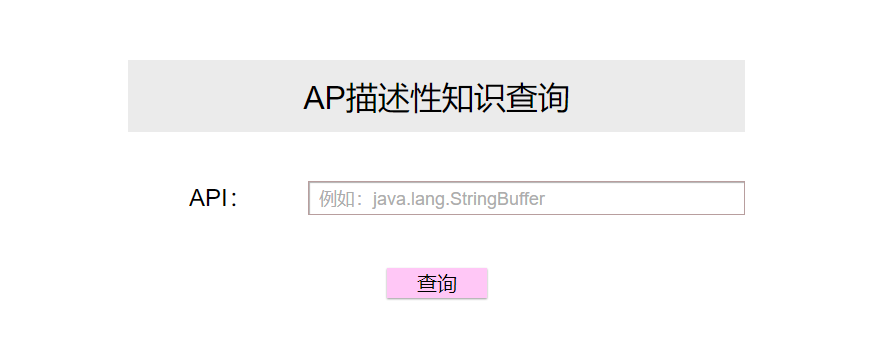
\includegraphics[width=\textwidth]{image/input.png}
    }
    \subfigure[展示界面]{
        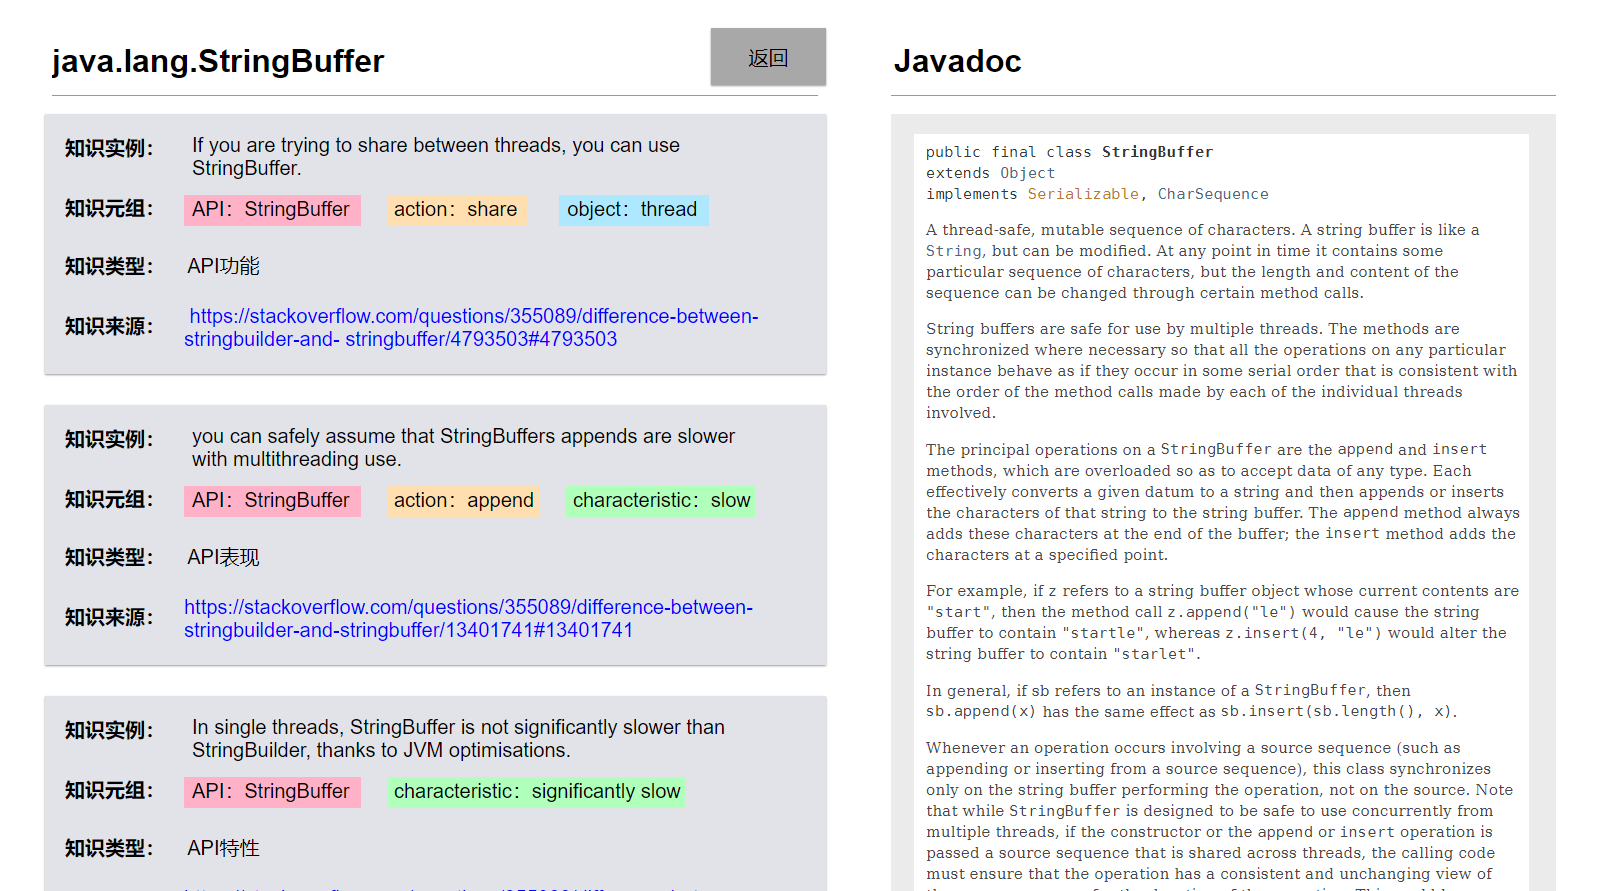
\includegraphics[width=\textwidth]{image/output.png}
    }
    \caption{知识汇总应用前端} 
    \label{fig:fig1} 
\end{figure}

\section{本章小结}
本章介绍了API描述性知识抽取系统及其应用的设计和实现。其中,抽取系统设计为三个模块,分别是语料库生成模块,抽取主体模块以及知识图谱构建模块。本文的应用基于Flask框架、Gunicorn服务器以及Vue框架,实现了一个查询API描述性知识以及相关的API文档的应用。在下一章中,将会对整个系统进行实验评估,以验证本方法的有效性。


\chapter{实验评估}
章节3和章节4详细介绍了本文提出的方法及其系统设计与实现,最后实现了一个能够从Stack Overflow帖子中识别出API描述性知识句子,并从中迭代抽取API描述性知识的系统。为了对本文提出的方法进行多方面的评估,本章节将会介绍本文设计的一系列实验,以及实验的结果。本章节设计的实验主要是为了回答以下3个问题:
\begin{enumerate}
    \item RQ1:API描述性知识抽取系统中的各个模块工作效果如何,其输出质量如何?
    \item RQ2:从不同的方面对本方法抽取出来的API描述性知识进行评估,其有效性如何?
    \item RQ3:本方法抽取出来的API描述性知识能否对API文档进行补充。
\end{enumerate}

\section{语料库生成模块质量评估}
本章节将对API描述性知识抽取系统中的语料库生成模块进行实验评估。

\subsection{实验设计}
本节所设计的实验用于评估用于语料库的质量,评估重点在训练的fastText二分类器能否正确的识别出Stack Overflow中的API描述性知识句子。本文从完成分句后经过过滤的带有API提及的句子列表中随机采样2000个句子,并邀请了两位具有3年以上Java开发经验的硕士研究生,对这些句子进行独立标注,判断这些句子是否是API描述性知识句子。对于两位标注者的标注结果中不同的部分,邀请第三位标注者对这些不同的部分进行仲裁,并将仲裁结果作为最终的标注结果。

句子标注的结果如表\ref{fig:fig1}所示。在完成句子标注后,本文还需要对两位标注者的共识率进行检验。本文计算出两位标注者的Cohen's kappa指数,用于表示两位标注者的共识率。其计算方法如公式5.1所示:

\begin{equation}
    k=\frac{p_{o}-p_{e}}{1-p_{e}}
\end{equation}

其中,$p_{o}$为实际共识率,$p_{e}$为理论共识率。根据标注数据计算得出的Cohen's kappa系数为0.86,因此我们可以认为两位标注者对于API描述性知识句子标注的共识基本是一致的。

\begin{table}[h]
    \centering
    \caption{API描述性知识句子标注结果}
    \label{fig:fig1}
    \begin{tabular}{|l|l|l|l|}
    \hline
          & 标注者1 & 标注者2 & 仲裁结果 \\ \hline
    正样本数量 & 533  & 580  & 542  \\ \hline
    负样本数量 & 1467 & 1420 & 1458 \\ \hline
    \end{tabular}
    \end{table}

如前文章节4.1.3所述,在得到标注数据后本文还会使用nlpaug工具进行数据扩充,以保证标注数据训练出来的文本分类器的有效性。

在完成扩充后,本方法得到了正样本1626条,负样本1458条,共3084条数据。接着,使用十折交叉验证法来验证使用这些数据训练得到的文本分类器是否有效。十折交叉验证法将会把所有标注数据分为10份,分别取其中一份作为测试集,剩余九份作为训练集,训练10次从而得到十个模型,然后使用各自的测试集来测试十次训练得到的模型的准确度。十折交叉验证得到的召回率、准确率和F值如表\ref{fig:fig2}所示。

\begin{center}
    \begin{table}[h]
        \centering
        \caption{十折交叉验证数据结果}
        \label{fig:fig2}
        \begin{tabular}{cccccccccccc}
        \hline
        模型  & 1    & 2    & 3    & 4    & 5    & 6    & 7    & 8    & 9    & 10   & 平均值  \\ \hline
        准确率 & 0.74 & 0.75 & 0.75 & 0.77 & 0.73 & 0.74 & 0.75 & 0.75 & 0.76 & 0.74 & 0.75 \\
        召回率 & 0.79 & 0.80 & 0.80 & 0.87 & 0.81 & 0.81 & 0.81 & 0.80 & 0.80 & 0.79 & 0.81 \\
        F值  & 0.77 & 0.78 & 0.78 & 0.81 & 0.77 & 0.77 & 0.78 & 0.78 & 0.78 & 0.76 & 0.78 \\ \hline
        \end{tabular}
        \end{table}
\end{center}


\subsection{实验结果分析}
从十折交叉验证的结果来看,fastText二分类器的分类效果较好,平均分类准确率达到75\%,平均召回率达到了81\%。在本方法中,对于分类器分类错误的情况,本文更希望是一个负样本被识别为正样本,而不是相反的情况。这是因为文本分类器对语料库只是进行一个挖掘前的初筛,如果一个非API描述性知识句子被加入语料库中,它有可能在挖掘过程中完全没有被匹配上,这样对本方法的抽取结果就不会造成影响。而如果一个API描述性知识句子被分类成负样本,那么本方法就完全没有机会抽取到这个句子中包含的API描述性知识,同时还无法抽取得到它的语言模式及其变异,这对于本方法是一种损失。从以上实验数据中可以得知,该分类模型的召回率比准确率更高,而召回率通常用于衡量一个分类器对正样本的识别能力,准确率通常用于衡量分类器对负样本的区分能力。因此,可以认为该模型在本方法中对正样本的识别能力是较为出色的。

对fastText二分类器分类错误的数据进行分析,主要原因有:
\begin{enumerate}
    \item 句子中出现了API描述性知识句子中的高频词。如“I override the getPreferredSize() to return the appropriate dimension.”,这个句子包含了常在API描述性知识句子中出现的词汇“override”和“return”,但这个句子的语义更倾向于描述作者的行为,而非API的表现知识,故它虽然不是一个API描述性句子但被分类成了正样本。
    \item 分句错误导致的低质量句子分类错误。如“A ReentrantLock is owned by the thread last successfully locking, but not yet unlocking it.A thread invoking lock will return, successfully acquiring the lock, when the lock is not owned by another thread. The method will return immediately if the current thread already owns the lock.”,由于原帖子的作者在编写时对标点符号的使用较为随意(没有在句号后面加上空格),导致本文修改后的spaCy解析工具将整段话作为一个完整的句子,句子的长度过长,且没有出现非常明显的特征词汇,所以虽然其中存在API描述性句子,但仍然被分类成负样本。
\end{enumerate}

\subsection{语料库质量评估实验总结}
通过以上实验评估,可以认为本系统中的语料库生成模块的性能较好,能够作为API描述性知识抽取的基础。高质量的语料库一定程度上提高了抽取主体模块的输出质量。当语料库中的一个句子能够和抽取主体模块输入的种子API描述性知识元组匹配上,或者与其他API描述性知识句子的语言模式相似时,它是一个有效的API描述性知识的可能性非常高。限制提高语料库质量的瓶颈主要在训练数据的质量和自然语言处理工具上,如果之后能将文章语法不够严谨的帖子筛选掉,或者定制更智能的自然语言分句规则,那么fastText二分类器的分类效果或许能有所提升。

\section{抽取主体模块质量评估}
本章节将对系统中的抽取主体模块进行质量评估。

\subsection{实验设计}
为了验证抽取主体模块的有效性,本实验从句子语料库中随机采样了50个句子,其中35个是API描述性知识句子,另外15个句子不是API描述性知识句子,但在句子中包含有API提及。然后人工总结出这35个句子的API描述性知识元组,从其中随机选择5个作为种子API描述性知识元组,再将这些句子和种子知识元组作为抽取主体模块的输入,进行迭代抽取。抽取过程中,每一轮的抽取结果都会被保存下来,直到程序无法从语料库中抽取出新的知识元组和知识实例为止。通过观察对比每一轮抽取的结果与人工总结的API描述性知识元组,可以对本模块的输出质量进行评估。

\subsection{实验结果分析}
本实验每一轮迭代运行中抽取出来的API描述性知识数量如表\ref{fig:fig3}所示。在第4轮抽取的时候,没有新的API描述性知识元组被抽取出来,抽取流程终止。从抽取出来的知识元组数量分析,从5个种子API描述性知识出发经过3轮迭代可以抽取得到16个的新的知识元组。在结果中,还存在着从非API描述性知识句子中抽取出了错误的API描述性知识元组,这种错误的知识元组有2个。去掉错误的API描述性知识元组,可以计算得出本模块对测试数据的抽取覆盖率为14/30=0.47。

\begin{table}[h]
    \centering
    \caption{抽取主体模块质量评估实验结果}
    \label{fig:fig3}
    \begin{tabular}{|l|l|l|l|l|l|}
    \hline
    迭代轮次    & 起始 & 1 & 2  & 3  & 4  \\ \hline
    API描述性知识元组数量 & 5  & 8 & 12 & 21 & 21 \\ \hline
    API描述性知识实例数量 & 5  & 8 & 12 & 21 & 21 \\ \hline
    语言模式数量  & 0  & 8 & 10 & 18 & 18 \\ \hline
    \end{tabular}
    \end{table}

由于语料库和种子API描述性知识元组较少,基于概念的变异和基于语言模式变异时得到的潜在知识元组及语言模式有限,在本实验中得到一个覆盖率较低的结果是可以理解的。显然,当系统在大规模的语料库中运行时,由于API描述性知识元组和从API描述性知识实例中总结的语言模式变异后能匹配上更多的API描述性知识实例,会让下一迭代轮次的种子API描述性知识元组也更多,抽取覆盖率会大大提高。前文章节4.3.2中的知识图谱构建结果也支持这一结论。



对从API描述性知识句子中抽取出来的14个API描述性知识元组,将它们与同一句子中人工总结出来的知识元组进行比较。我们发现,抽取出来的知识元组中,与人工总结的知识元组组成元素完全相同的较少,只有4个,而与人工总结的知识元组至少有一个除API元素以外的相同元素的抽取结果更多,有12个。这是因为同一个API描述性知识元组可能有不同的抽取路径,可以通过不同的变异方式抽取出来,而且同一个句子可能可以用多个不同的API描述性知识元组来描述。

\subsection{抽取主体模块质量评估实验总结}
通过设计以上实验并验证,可以认为本系统的抽取主体模块可以正常地从给定的语料库中抽取出API描述性知识实例,且在语料库较大的时候表现更好,覆盖率更高。抽取出来的API描述性知识元组中,大部分结果与人工总结的知识元组至少包含一个相同的元素,说明抽取模块对API描述性知识的抽象与人工总结的结果是相似的。综上,可以认为本系统中的抽取主体模块是有效的。

\section{API描述性知识的有效性评估}
在本章节中,将会对本系统抽取得到的API描述性知识进行有效性评估。

\subsection{实验设计}
为了对本系统抽取出来的API描述性知识进行评估,首先从本文构建的知识图谱中随机抽取出100条API描述性知识元组及其实例,依然邀请两位具有3年Java开发经验的硕士研究生进行该实验。两位实验参与者会对这100条API描述性知识进行阅读、打分。API描述性知识元组及其实例的表示如图\ref{fig:fig1}所示。参与者会从以下三个方面进行评分:

\begin{figure}[htb]
    \centering
    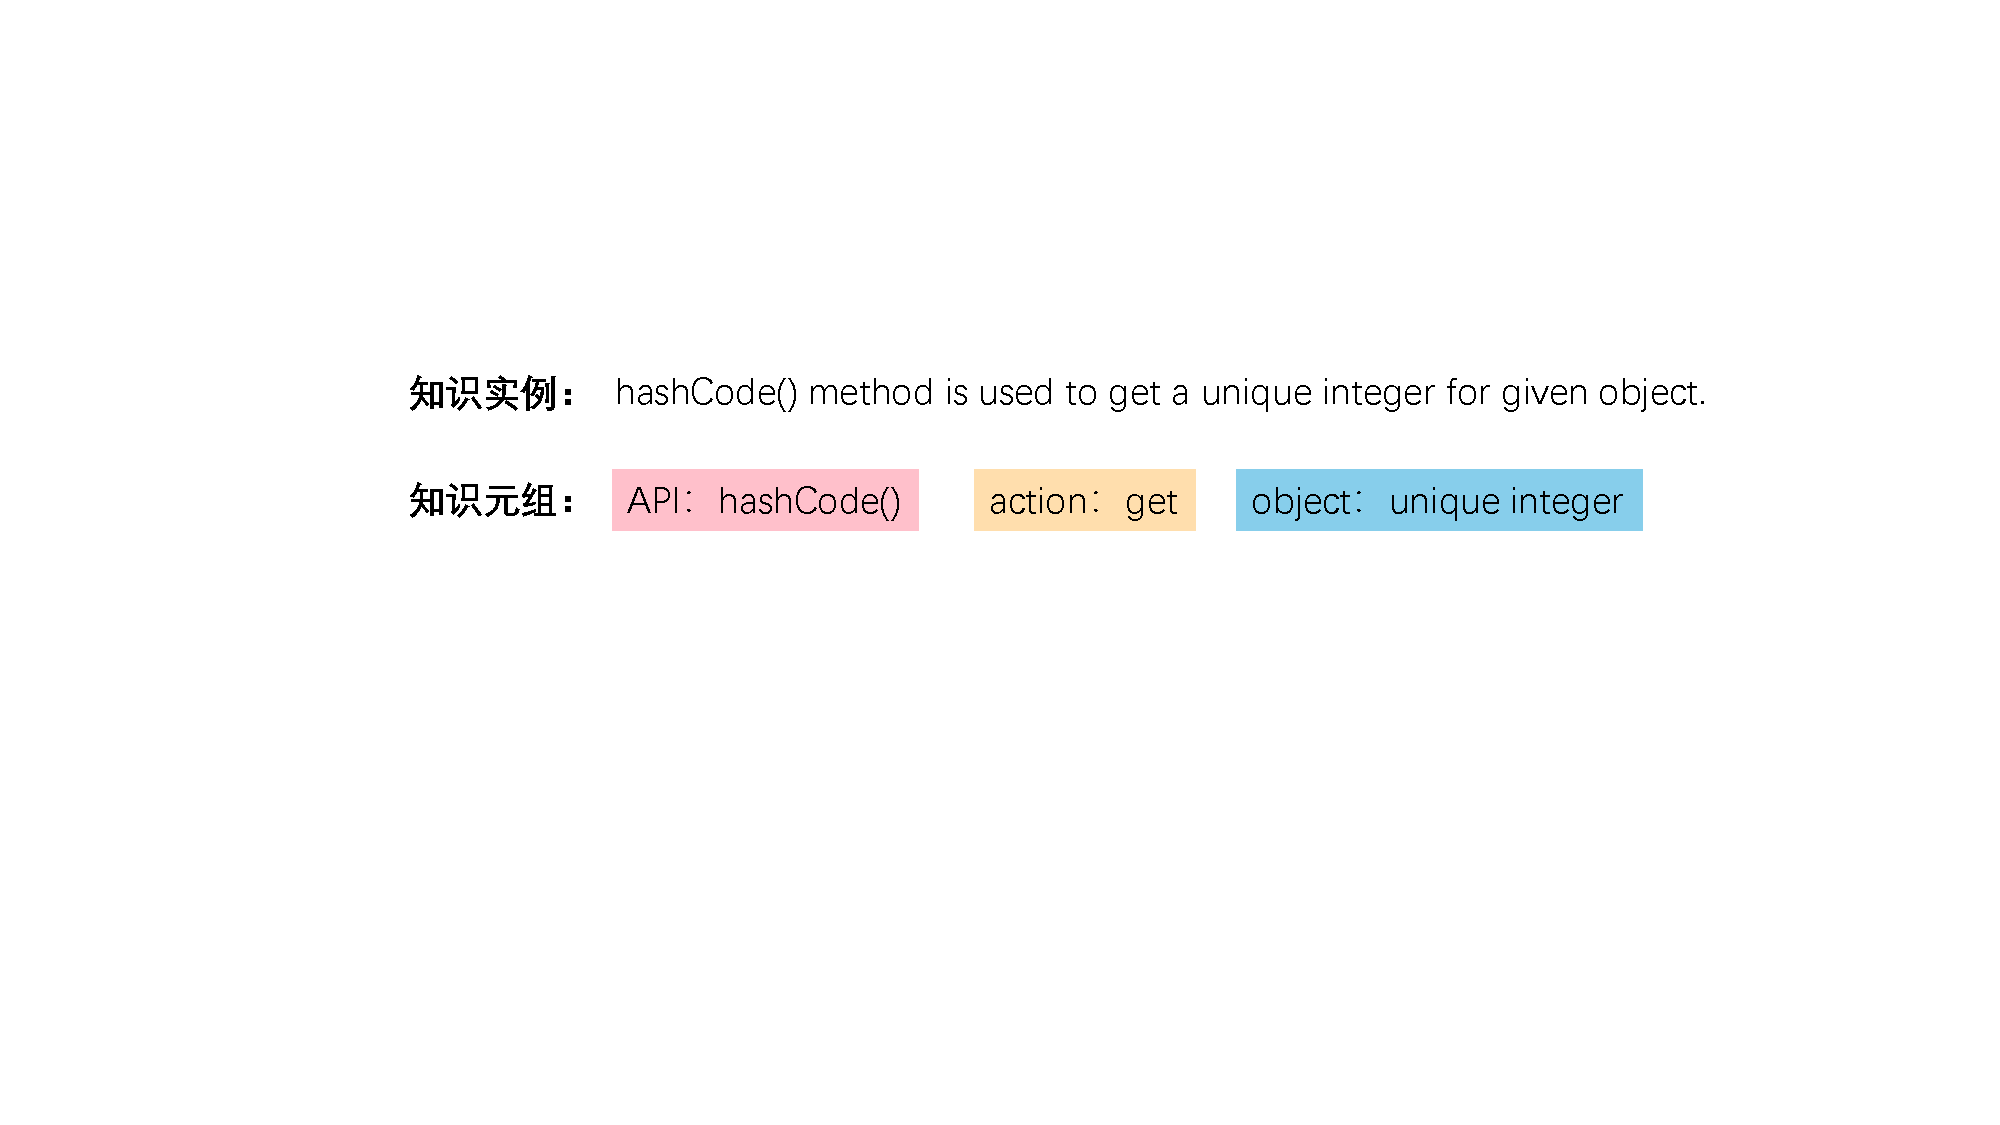
\includegraphics[width=\textwidth]{image/instance.pdf}
    \caption{API描述性知识元组及其实例示例} 
    \label{fig:fig1} 
\end{figure}

\begin{itemize}
    \item 完整性:这个实例是否完整地描述了一个API描述性知识,没有缺失必要的信息。
    \item 有用性:掌握这个API描述性知识是否对软件开发有所帮助,是否能在软件开发的过程中使用到。
    \item 可理解性:这个API描述性知识元组是否能让人快速的理解完整的API描述性知识实例。
\end{itemize}
评分从0分到3分,0分表示非常不同意,1分表示部分不同意,2分表示部分同意,3分表示非常同意。

\subsection{实验结果分析}
图\ref{fig:fig2}为本章节实验的评分结果。在本章节的实验中,综合两位标注者对于API描述性知识的完整性评分,有26\%的评分为3分,59\%的评分为2分,而负面评价的1分和0分分别占12\%和3\%。对于API实例的有用性评分,32\%的评分为3分,53\%的评分为2分,评分为1分的有13\%,剩余2\%的评分是0分。而在可理解性方面,正面评分的3分和2分的比例分别是7\%和58\%,负面评价的1分和0分的比例则为28\%和7\%。两位参与者在完整性、有用性、可理解性三个方面的平均评分分别为2.08、2.16、1.58和2.08、2.14、1.72。	

\begin{figure}[htb]
    \centering
    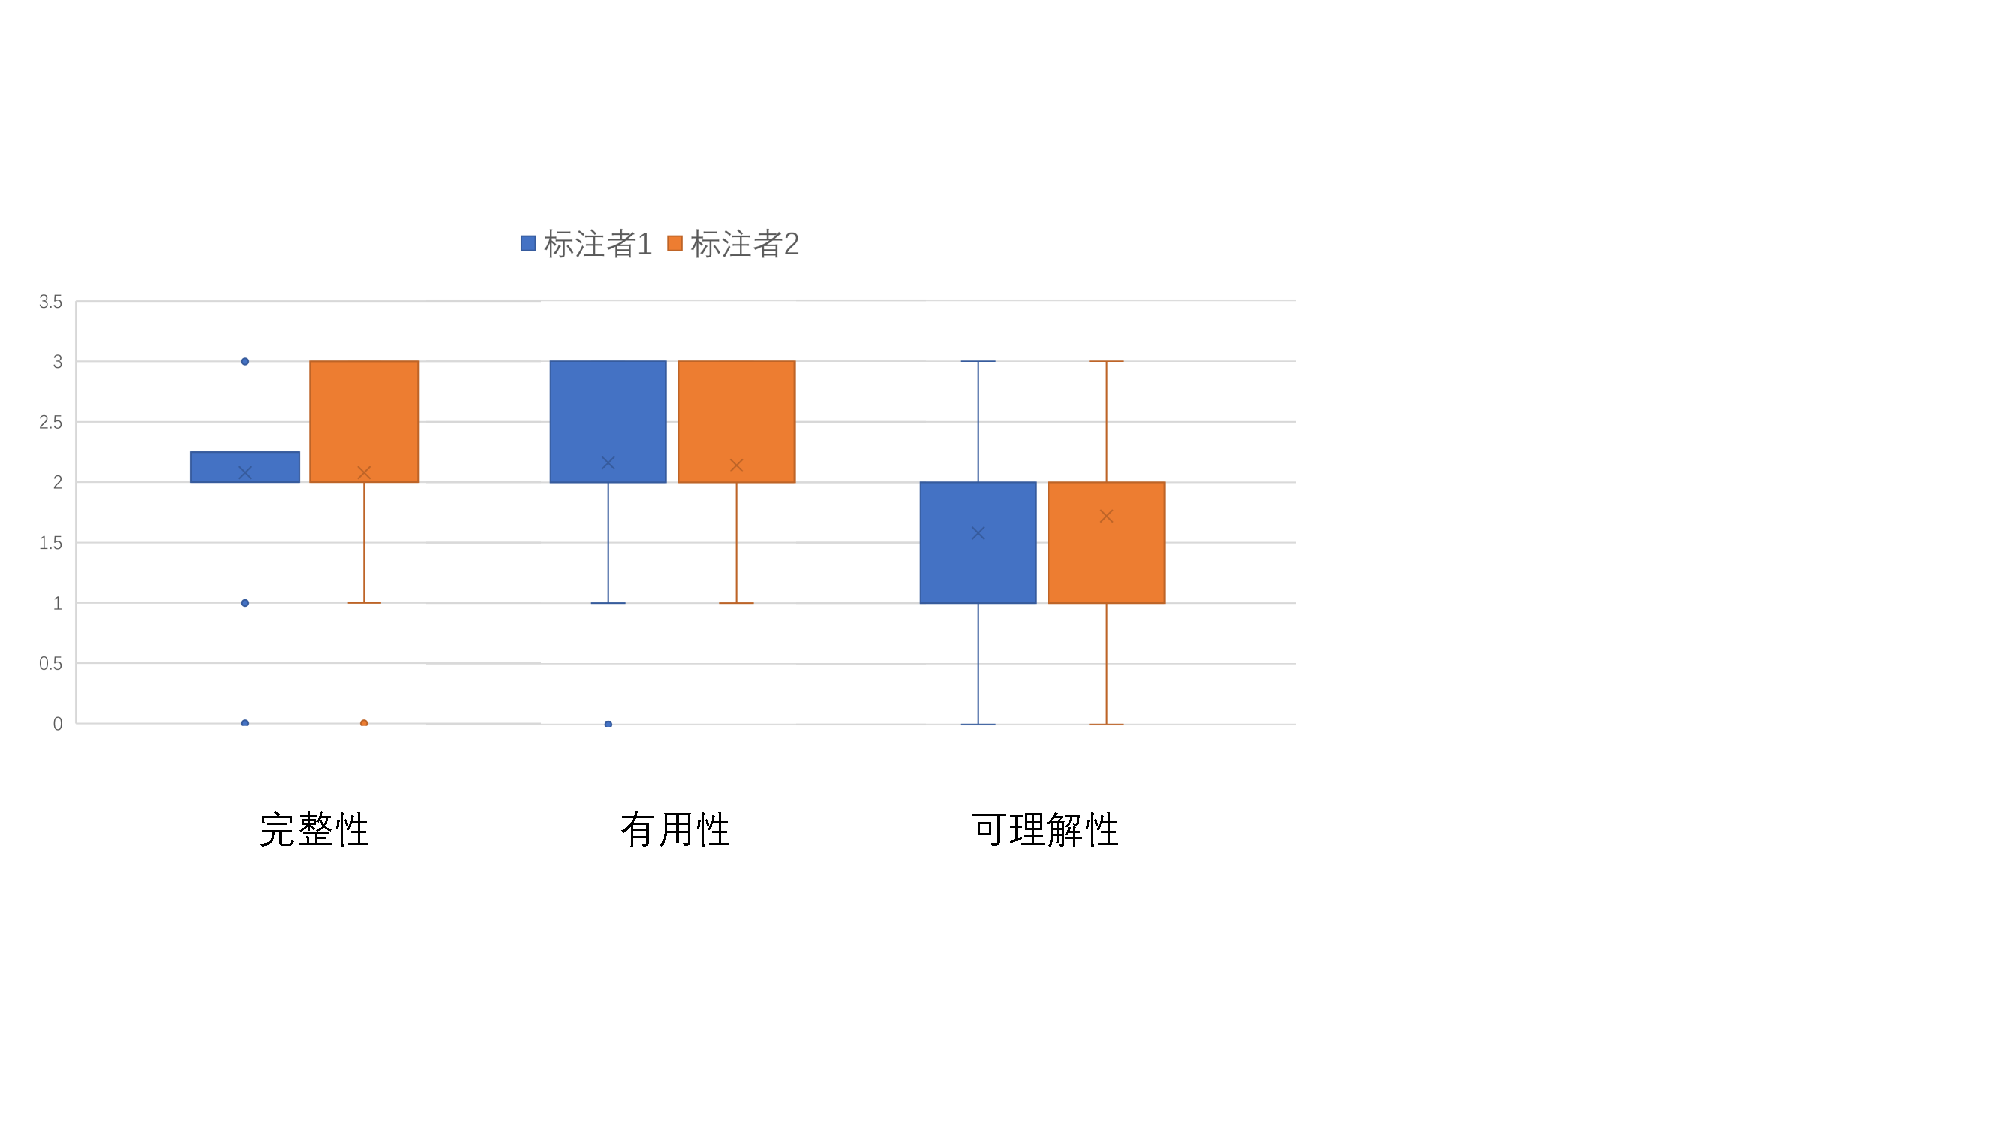
\includegraphics[width=\textwidth]{image/youxiaoxing.pdf}
    \caption{API描述性知识有效性评估实验结果} 
    \label{fig:fig2} 
\end{figure}

为了保证两位参与者的打分情况的显著性差异,本文对两位参与者的评分数据进行了双样本的T检验。在T检验的结果中,如果显著性水平值p<0.05,则可以说明两组数据之间存在显著的差异。而在本章节的实验结果中,计算得到的显著性水平值p为0.047,小于0.05,因此两组数据之间确实是存在显著性差异的。

从以上数据中可以得知,本方法抽取得到的API描述性知识实例在完整性、有用性方面是较为优秀的,平均评分达到了2.08和2.15,说明实验参与者认为本方法抽取出的API描述性知识实例在软件开发的过程中能够有效地帮助到程序员。

对实验数据中完整性和有用性被评为0分的API描述性知识实例进行分析,本文发现它们主要有以下特点:

\begin{enumerate}
    \item 实例中同时包含多个动作元素以及多个目标对象元素。由于本方法中的知识元组匹配环节中,只要一个句子中包含知识元组中的所有元素,就可以匹配得到一个知识实例,所以一个缺失元素的知识元组也有可能匹配上一个知识实例。
    \item 实例中描述的知识内容不完整。由于本文实现的是句子级别的API描述性知识抽取,所以本方法对一个由多个句子组成的API描述性知识的抽取效果较差。当遇到这种多句子API描述性知识时,本系统只能抽取出残缺的知识,这些知识的有用性较差。
\end{enumerate}

针对上述第一个问题,可以考虑在抽取出API描述性知识实例后,基于实例中的词语对匹配的API描述性知识元组进行补全。这样就能有效提高本文抽取出来的API描述性知识的完整性。针对第二个问题,如果未来能实现将细粒度和粗粒度的知识抽取方式相结合的抽取方法,可以克服这一缺点。

而在可理解性方面,本方法抽取出的API描述性知识元组的可理解性较为一般,因为一个完整的API描述性知识句子的语义较为复杂,而本方法抽取出的API描述性知识元素数量有限,且没有上下文信息,这种抽象化的结构表达对于人来说是比较难理解的。但抽象化的结构表达对于帮助机器理解语义有非常大的帮助,且结构化的API描述性知识元组能帮助本系统构建成带有层次关系的知识图谱,便于通过API知识元素和API描述性知识元组之间的关系进行检索。如在本文构建得到的API描述性知识图谱中,只要搜索所有与“thread-safe”这个characteristic之间有has characteristic关系的API描述性知识及其实例,就能实现对thread-safe这个API特性的范围检索,找到所有带有thread-safe特性的API。

\subsection{API描述性知识的有效性评估实验总结}
通过上文中的实验分析,我们可以认为本方法中抽取出来的API描述性知识实例在完整性、有用性方面较为优秀,抽取出来的API描述性知识元组也能够在软件开发的过程中对程序员有所帮助,且API描述性知识元组的结构化表达也为本系统构建知识图谱提供了帮助,方便根据图谱中的关系进行检索。

\section{API描述性知识汇总应用对API文档的互补性评估实验}
在验证完本方法抽取出来的API描述性知识的有效性基础之上,本章节将继续讨论这些知识能否对API文档进行补充。章节4.4介绍了本文实现的API描述性知识汇总应用,本章节设计的实验将邀请开发者使用该应用,并对该应用给出的API描述性知识是否能对API文档完成补充进行评价。

\subsection{实验设计}
首先从本文中构建的API描述性知识图谱中检索出包含API描述性知识实例数量大于10条的API节点,共有309个,在其中随机选择20个作为目标API。然后依旧是邀请两位硕士研究生,请他们使用本文实现的汇总应用查询目标API,并判断系统左侧展示的API描述性知识实例能否作为系统右侧展示的API文档的补充知识。系统的具体展示页面详见图4-1。

本实验的内容同样是对API描述性知识实例进行打分,要求两位实验参与者对系统左侧展示的前五条API描述性知识实例评分,即一共对100条API描述性知识实例进行评估。打分的标准从0到3分,0分表示完全无法作为API文档的补充,1分表示这条API描述性知识实例已经包含在API文档里了,2分表示API描述性知识实例中的部分表述可以作为文档的补充,3分表示这个知识实例可以完整地补充到API文档中。

\subsection{实验结果分析}
实验结果统计如图\ref{fig:fig3}所示。综合两位标注者的评分结果来看,有19.5\%的评分是3分,49\%的评分是2分,标注为1分的评分有22\%,最后还有9.5\%的API描述性知识实例被评为0分。所有API描述性知识实例的平均评分是1.785。单独对每一个随机选取的API来看,每个API相关的5条API描述性知识实例中,平均有0.98条知识实例被评为3分,2.45条知识实例被评为2分,作为负面评价的1分和0分分别有1.1条和0.48条。从实验结果中可以得知,本方法抽取出来的API描述性知识对于API文档具有良好的补充作用,随机采样得到的100条API描述性知识实例的平均评分为1.785,表示这些知识实例大多是对于补充API文档具有正面作用的。

\begin{figure}[htb]
    \centering
    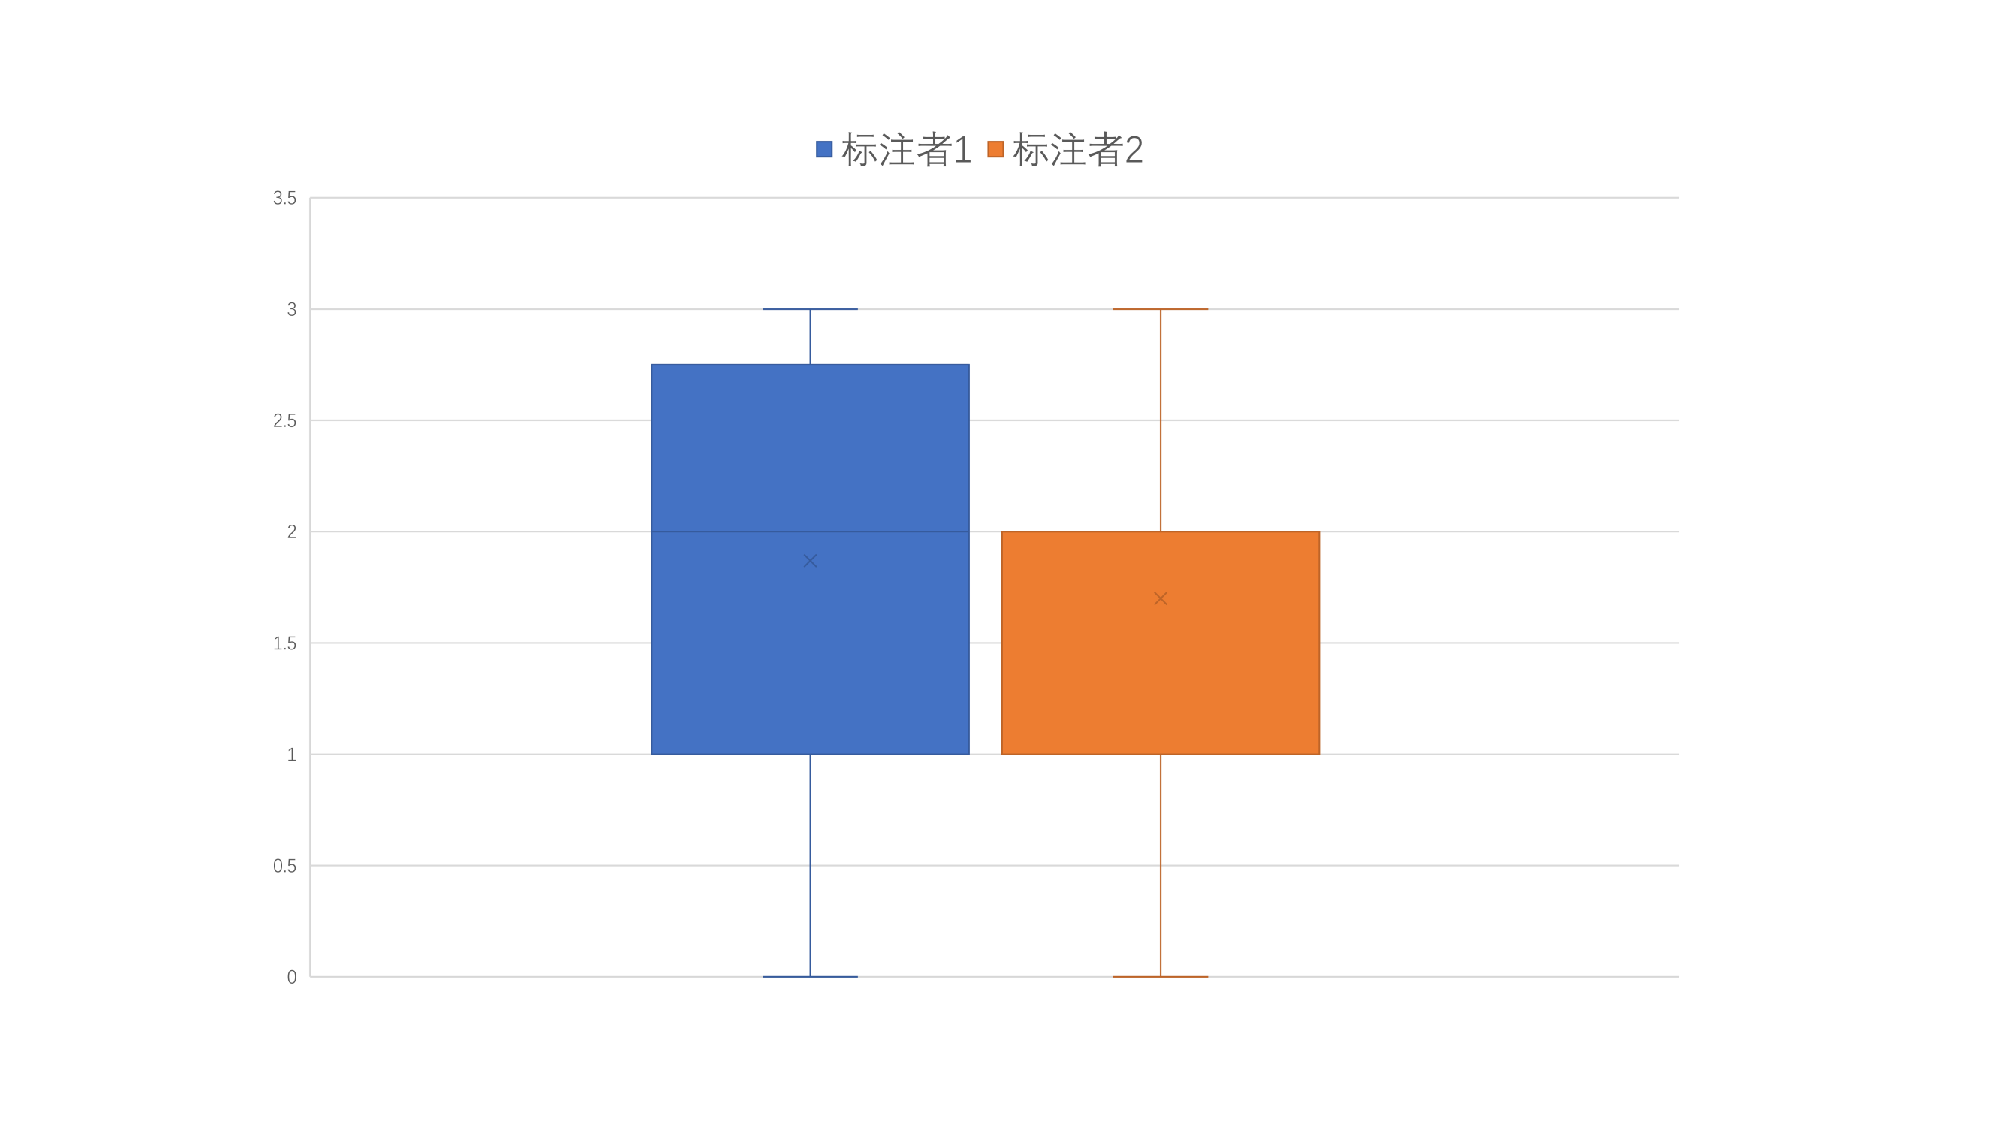
\includegraphics[width=\textwidth]{image/5-2.pdf}
    \caption{API描述性知识汇总应用与API文档互补性评估实验结果} 
    \label{fig:fig3} 
\end{figure}

由于本方法在进行API描述性知识的抽取之前,对语料库进行了多项过滤工作,保证了语料库中API描述性知识句子的覆盖率,所以本方法抽取得到的API描述性知识的有效性是具有保障的,前文章节5.3所设计的实验也证明了这一点。但在本系统抽取得到的知识中,部分API描述性知识来自于原作者在帖子中引用API文档中已有的知识,或者用自己的语言重新描述一个API文档中已存在的知识点,这种API描述性知识在本方法的挖掘结果中占了22\%。

除此之外,实验结果中还存在49\%的API描述性知识实例被评为2分。这些知识实例既包括了API文档中已有的知识点,也存在部分不在API文档之中的知识。开发者们在Stack Overflow上讨论一个API时,可能会加上自己对这个API的理解,或者对已有的API知识进行深入的拓展讨论,比如分析一个API的特性是如何在底层实现的。我们认为这种API描述性知识实例对于API文档的补充是具有正面价值的。

对于这些与API文档包含有重复知识的API描述性知识实例,如果能基于API文档本身对本系统抽取出来的知识实例进行过滤,那么剩余的知识实例的有效性将会大大提升。可以考虑使用基于句子相似度的过滤方式对本文抽取出来的知识实例进行去重,如对API文档进行分句,然后计算API描述性知识实例与文档中的每一个句子的句子相似度。如果该实例与API文档里的其中一个句子相似度很高,就将这个实例过滤掉。这样经过过滤后,本系统实现的应用对于API文档的互补性应该会大大提升。

最后,由于API文档对一个API的表述非常简洁,只取重点,大多数API文档仅仅是对API的功能、输入以及输出进行介绍。而在Stack Overflow上,开发者们对一个API的讨论可能会深入到源码层面,或者对一个API在实际编程过程中的表现、特性等进行讨论,所以本文方法能够在这种讨论中抽取出不存在于API文档中的知识。

\subsection{API描述性知识汇总应用的有效性评估实验总结}
本章节设计的有效性评估实验证明了本方法抽取出来的API描述性知识实例大多对API官方文档的补充具有一定的价值。其中,部分API描述性知识实例已经被API文档覆盖了,如果能够提出一种过滤机制对抽取出来的API描述性知识再进行一次筛选,过滤掉那些已经在文档中存在的知识,那么本方法抽取出来的API描述性知识的价值将会大大提高。

\section{方法有效性威胁}
本方法的有效性威胁主要分为两个部分,分别是存在于本文方法之中的内部有效性威胁和除此之外的外部有效性威胁。

\subsection{内部有效性威胁}
在本文的知识抽取流程中,面临的内部有效性威胁来自于本方法所使用的一些外部工具,包括fastText文本分类器和自然语言处理工具spaCy。在生成语料库的时候,本方法使用了fastText文本分类技术,用于从包含API提及的句子中识别出API描述性知识句子。尽管fastText分类器的文本分类效果很好,但仍不能达到100\%的分类准确率。当一个非API描述性知识句子被分类为正样本时,这个句子可能在抽取过程中并不会被匹配上,也可能会从这个句子中抽取出错误的API描述性知识元组。而在本文的抽取流程中,一个错误的抽取结果会像一个雪球一样在多次迭代后越滚越大,形成更多错误的知识和语言模式,这样会对本方法抽取得到的结果产生不良影响。为了保证本方法的有效性,本文在抽取流程中设置了严格的过滤条件,用于筛选掉错误、低质量的API描述性知识元组。本文的实验评估证明过滤机制是有效的,但分类错误带来的影响依然部分存在于抽取结果中。

而自然语言处理工具spaCy的性能也对本方法的有效性有着举足轻重的影响。spaCy在自然语言解析的过程中出现的分词、分句错误都会对本方法带来负面影响。虽然spaCy的性能在自然语言处理领域是非常优秀的,且它在被应用于软件工程相关文本的时候相比其他工具有着更好的表现,但目前也并没有哪个自然语言处理工具能够在处理大规模语料时保证100\%的准确率。本文方法中,Stack Overflow帖子的分句依赖于spaCy的句子解析模块,API描述性知识实例的语言模式抽取也依赖于spaCy的词语解析模块。虽然本方法使用了贴近于Stack Overflow网站文本的定制化分句、分词规则,且在语言模式匹配时将单词数量阈值设置为4个以提高分词容错率,但依然会因为文本自身的一些问题导致分词分句的错误(如前文章节5.1.2所述),以及语言模式抽取的错误。

\subsection{外部有效性威胁}
本文面对的外部有效性威胁主要来自于实验评估环节,以及方法的泛用性相关问题。
在实验评估环节中,本文设计的部分实验具有较强的主观性,且实验的规模较小。如章节5.3以及章节5.4所设计的实验,均采用了人工评分的方式来对本文抽取的结果进行评估,而且抽样的实例数量只有100条。为了减轻实验参与者的主观性对本方法造成的影响,本文邀请的标注者首先要求具有3年以上的Java语言开发经验,这确保了他们对于Java语言的API知识是足够熟悉的。其次,本文在实验部分均至少邀请了两位参与者,并且在得到实验结果后设计了T检验对结果进行检查,确保两人的评分结果是存在显著性差异的。但实验规模较小带来的有效性威胁仍然是客观存在的。

此外,由于本方法的语料库生成模块只选用了带有Java标签的Stack Overflow帖子,且实验评估也是针对Java语言所设计的,并没有对其他的编程语言帖子进行抽取和实验,所以还不能确保本方法在其他编程语言上具有泛用性。

\section{本章小结}
本章节中,首先提出了3个问题,分别从系统流程的有效性以及系统产出的有效性两个方面入手进行讨论,并设计了一系列实验,分别验证了本文流程中语料库生成模块与抽取主体模块的有效性以及本文方法抽取出的API描述性知识实例的有效性。对于本文实现的API描述性知识汇总应用,本文还设计了与API文档的补充实验,证明本文方法抽取得到的部分API描述性知识实例能够作为API文档的补充,是具有一定价值的。在本章的最后,还对本文面临的内部有效性威胁和外部有效性威胁进行了讨论。


\chapter{总结与展望}
本章节是对本文提出的方法的总结以及对未来工作的展望。
\section{本文总结}
现代软件开发过程中,开发者常在程序开发领域的知识问答网站如Stack Overflow上讨论与API相关的话题,在API官方文档无法满足程序员的学习需求时,Stack Overflow成为了开发者们获取知识的最佳途径。因此,针对Stack Overflow的API知识挖掘技术应运而生。在之前的研究中,有些学者使用基于规则的方式进行知识挖掘,有些学者则是采用了基于机器学习的方法进行挖掘,均能在特定场景下取得不错的效果,但也都有它们的不足之处。本文针对这一课题提出了新的想法,设计了一种基于自举思想的API描述性知识抽取方法,通过结合目前较为成熟的基于机器学习的文本分类技术和基于规则的知识抽取方法,从Stack Overflow中迭代地抽取出API描述性知识。

现代文本分类技术已经非常成熟且易用,本文使用了Facebook公司开源的fastText文本分类技术,并结合人工制定的规则,对Stack Overflow上的文本句子进行筛选,识别出其中的API描述性知识句子,再在这些句子组成的语料库中进行基于概念变异的API描述性知识实例抽取和基于语言模式变异的API描述性知识元组抽取。对于抽取得到的API描述性知识及其实例,本文还将其构建成一个API描述性知识图谱,并基于知识图谱实现了一个API描述性知识汇总应用。在信息检索方面,图数据库比关系型数据库更为高效、直观。

最后,本文还设计了一系列实验对本方法进行评估,针对本方法的语料库生成模块、抽取主体模块进行了质量评估,并对抽取出来的API描述性知识的有效性以及对API文档的互补性进行了评估。实验结果表明,本文提出的方法抽取得到的API描述性知识具有一定的价值,且能对API文档起到补充作用。
\section{未来展望}
本文提出的方法虽然能从给定的语料库中抽取出API描述性知识,但仍然有缺陷。本文方法可以改进的地方有:
\begin{enumerate}
    \item 本文方法部分依赖于spaCy的性能,虽然本文针对Stack Overflow上的文本特点进行了部分优化,但是依然会有解析错误的情况出现,故未来的一个工作方向可以是针对软件开发相关的自然语言处理继续进行优化,实现更好的解析效果。
    \item 本文只选取了带有Java标签的Stack Overflow帖子作为知识挖掘的语料,而Stack Overflow上还有其他热门语言标签如Python、PHP、JavaScript等,接下来的工作可以专注于提高本方法的泛用性,将API描述性知识的抽取从Java语言拓展到其他语言中。
    \item 本方法进行抽取后构建的API描述性知识图谱结构还比较简单,对API描述性知识的分类也只有三种,而对API知识进行分类这一工作国内外许多学者都有做过相关的研究,所以下一步的工作可以是结合本文方法,对抽取出来的API描述性知识进一步的细分归类,构建更加精细的API描述性知识图谱。
\end{enumerate}

% 后置部分包含参考文献、声明页(自动生成)等
\backmatter

% \fancyhead{}
% \fancyhead[L] { \small \nouppercase { \fdu@kai \l_fdu_info_title_tl  } }
% \fancyhead[R] { \small 参考文献 }
% \renewcommand\refname{参考文献}
% \fancyhead{}
% \fancyhead[L]{\small 基于软件开发问答网站的API描述性知识抽取}
% \fancyhead[R]{\small 参考文献}
\renewcommand\refname{参考文献}

\bibliography{citelist}

\chapter{致谢}
% \addcontentsline{toc}{chapter}{致谢}
\input{section/thanks}

% 专硕同学可以注释


\end{document}
